% Options for packages loaded elsewhere
\PassOptionsToPackage{unicode}{hyperref}
\PassOptionsToPackage{hyphens}{url}
%
\documentclass[
  a4paper,
]{article}
\usepackage{amsmath,amssymb}
\usepackage{lmodern}
\usepackage{ifxetex,ifluatex}
\ifnum 0\ifxetex 1\fi\ifluatex 1\fi=0 % if pdftex
  \usepackage[T1]{fontenc}
  \usepackage[utf8]{inputenc}
  \usepackage{textcomp} % provide euro and other symbols
\else % if luatex or xetex
  \usepackage{unicode-math}
  \defaultfontfeatures{Scale=MatchLowercase}
  \defaultfontfeatures[\rmfamily]{Ligatures=TeX,Scale=1}
\fi
% Use upquote if available, for straight quotes in verbatim environments
\IfFileExists{upquote.sty}{\usepackage{upquote}}{}
\IfFileExists{microtype.sty}{% use microtype if available
  \usepackage[]{microtype}
  \UseMicrotypeSet[protrusion]{basicmath} % disable protrusion for tt fonts
}{}
\makeatletter
\@ifundefined{KOMAClassName}{% if non-KOMA class
  \IfFileExists{parskip.sty}{%
    \usepackage{parskip}
  }{% else
    \setlength{\parindent}{0pt}
    \setlength{\parskip}{6pt plus 2pt minus 1pt}}
}{% if KOMA class
  \KOMAoptions{parskip=half}}
\makeatother
\usepackage{xcolor}
\IfFileExists{xurl.sty}{\usepackage{xurl}}{} % add URL line breaks if available
\IfFileExists{bookmark.sty}{\usepackage{bookmark}}{\usepackage{hyperref}}
\hypersetup{
  pdftitle={Heterarchical Control in Sensorimotor Processing},
  pdfauthor={Spencer R. Wilson},
  hidelinks,
  pdfcreator={LaTeX via pandoc}}
\urlstyle{same} % disable monospaced font for URLs
\usepackage[margin=30mm]{geometry}
\usepackage{graphicx}
\makeatletter
\def\maxwidth{\ifdim\Gin@nat@width>\linewidth\linewidth\else\Gin@nat@width\fi}
\def\maxheight{\ifdim\Gin@nat@height>\textheight\textheight\else\Gin@nat@height\fi}
\makeatother
% Scale images if necessary, so that they will not overflow the page
% margins by default, and it is still possible to overwrite the defaults
% using explicit options in \includegraphics[width, height, ...]{}
\setkeys{Gin}{width=\maxwidth,height=\maxheight,keepaspectratio}
% Set default figure placement to htbp
\makeatletter
\def\fps@figure{htbp}
\makeatother
\setlength{\emergencystretch}{3em} % prevent overfull lines
\providecommand{\tightlist}{%
  \setlength{\itemsep}{0pt}\setlength{\parskip}{0pt}}
\setcounter{secnumdepth}{5}

%% pandoc-fignos: required package
\usepackage[capitalise]{cleveref}

%%%% pandoc-fignos: required package
\usepackage{caption}

%% pandoc-fignos: environment to disable figure caption prefixes
\makeatletter
\newcounter{figno}
\newenvironment{fignos:no-prefix-figure-caption}{
  \caption@ifcompatibility{}{
    \let\oldthefigure\thefigure
    \let\oldtheHfigure\theHfigure
    \renewcommand{\thefigure}{figno:\thefigno}
    \renewcommand{\theHfigure}{figno:\thefigno}
    \stepcounter{figno}
    \captionsetup{labelformat=empty}
  }
}{
  \caption@ifcompatibility{}{
    \captionsetup{labelformat=default}
    \let\thefigure\oldthefigure
    \let\theHfigure\oldtheHfigure
    \addtocounter{figure}{-1}
  }
}
\makeatother
\ifluatex
  \usepackage{selnolig}  % disable illegal ligatures
\fi
\newlength{\cslhangindent}
\setlength{\cslhangindent}{1.5em}
\newlength{\csllabelwidth}
\setlength{\csllabelwidth}{3em}
\newenvironment{CSLReferences}[2] % #1 hanging-ident, #2 entry spacing
 {% don't indent paragraphs
  \setlength{\parindent}{0pt}
  % turn on hanging indent if param 1 is 1
  \ifodd #1 \everypar{\setlength{\hangindent}{\cslhangindent}}\ignorespaces\fi
  % set entry spacing
  \ifnum #2 > 0
  \setlength{\parskip}{#2\baselineskip}
  \fi
 }%
 {}
\usepackage{calc}
\newcommand{\CSLBlock}[1]{#1\hfill\break}
\newcommand{\CSLLeftMargin}[1]{\parbox[t]{\csllabelwidth}{#1}}
\newcommand{\CSLRightInline}[1]{\parbox[t]{\linewidth - \csllabelwidth}{#1}\break}
\newcommand{\CSLIndent}[1]{\hspace{\cslhangindent}#1}

\title{Heterarchical Control in Sensorimotor Processing}
\author{Spencer R. Wilson}
\date{\today}

\usepackage[capitalise]{cleveref}
\usepackage{graphicx}
\graphicspath{{/Users/spencerw/Google Drive/motor_control/phd/}}
\usepackage{subfigure}

\begin{document}
\maketitle

\hypertarget{sec:intro}{%
\section{Introduction \& Aims}\label{sec:intro}}

\begin{quote}
\emph{Movement is nothing but the quality of our being.}

--- Sunryu Suzuki, \emph{Zen Mind, Beginner's Mind}
\end{quote}

The purpose of this thesis is to build a high-dimensional
electromyography recording setup, and use this to produce a platform for
closed-loop motor control and learning experiments on which a suite of
tasks and perturbations can be tested. With this relatively novel setup,
we hope to advance our understanding of trial-to-trial motor learning by
testing new model predictions through mixture of experiment and theory.

Hans Moravec's eponymous paradox states that it is easier to generate
artificially intelligent performance on tasks we think of as
intellectually challenging, such as chess, than to provide a machine
with faculties we take for granted, such as movement. Moravec's Paradox,
for example, encourages us not to look past the complex computations
generated by the human motor system. Following Moravec, this work
focuses on what is arguably the most advanced control apparatus in the
known universe: the human movement machine.

A recent review provides a clear call to action for work this direction:

\begin{quote}
The processes by which biological control solutions spanning large and
continuous state spaces are constructed remain relatively unexplored.
Future investigations may need to embed rich dynamical interactions
between object dynamics and task goals in novel and complex
movements.\textsuperscript{\protect\hyperlink{ref-McNamee2019}{1}}
\end{quote}

Over the last few decades, there has been considerable amount of work
done to untangle the abilities of the motor system to flexibly control
the body including through optimal control
theory\textsuperscript{\protect\hyperlink{ref-Todorov2004}{2}},
reinforcement learning in continuous action
space\textsuperscript{\protect\hyperlink{ref-koberReinforcementLearningRobotics2013}{3}},
and detailed physiological
studies\textsuperscript{\protect\hyperlink{ref-sauerbreiCorticalPatternGeneration2019}{4}}.
However, as the quote above suggests, a holistic understanding of the
computations underlying the generation of skilled movement remains an
open problem. The aim of this thesis is to progress our understanding of
skilled movement by studying the solutions produced by human subjects to
motor tasks in dynamically rich, yet controlled, virtual environments.
Our goal is to reverse-engineer the ability to acquire and perform novel
motor skills. First we define what we mean by the terms \emph{skill},
and \emph{task}.

Humans produce a great variety of movements every day, often without
conscious thought. For example, movements like bringing a cup of coffee
to our lips for a sip are generally out of reach for state-of-the-art
robotic systems. We claim that this ``motor gap'' between biological and
artificial motor systems is due to a lack of \emph{dexterity} in the
latter. Soviet neuroscientist Nikolai Bernstein defined dexterity as the
ability to ``find a motor solution in any situation and in any
condition.''\textsuperscript{\protect\hyperlink{ref-Bernstein1967}{5}}
The crux of this definition is the flexibility of such solutions. This
flexibility, or
robustness\footnote{Kitano defines robustness as ``the maintenance of
  specific functionalities of the system against perturbations, and it
  often requires the system to change its mode of operation in a
  flexible way.'' He claims that robustness requires control,
  alternative mechanisms, modularity and decoupling between high and low
  level variability.}\textsuperscript{\protect\hyperlink{ref-kitanoBiologicalRobustness2004}{6}},
is the ability to optimize internal parameters in response to external
perturbations and adapt to new information to achieve the goals of an
ongoing plan.

While a robot may be able to move a cup of coffee to a precise location
in space, its solution is often found to be brittle in a new context, or
unable to generalize to the movement of new objects. We define a skill
as a behavior that involves dexterity in Bernstein's sense. The use of a
tool such as a screwdriver is an example of a motor skill. We define a
task as the production of skilled movement in a particular context.
Driving a screw in a particular posture using a particular screwdriver
is an example of a task. These concepts will be further formalized in
later chapters.

Human movement is ultimately the result of the activation and
contraction of muscle fibers, and movements lie on a spectrum between
reflexive and volitional. The supramuscular circuitry which determines
the degree of volition we ascribe to movement, where volitional movement
relies on supraspinal (though not necessarily conscious) processes. The
human hand is a unique evolutionary invention that underlies our ability
to perform various skills in a range of tasks-- movements that are
decidedly volitional\footnote{It could be argued that the hand is in
  fact a crucial aspect of humanness. It is thought that the human
  cerebellar and neocortices evolved reciprocally to expand and support
  the computational burden of increasingly complex motor tasks such as
  tool-making and language production. REF?}. The hand is the pinnacle
of dexterity and, as such, it is a fruitful testbed for studying the
computations and circuitry that drive dexterous movement. A detailed
physiological review of the hand and it's relation to skilled movement
is described in \cref{sec:physiology}.

We are more interested in the leveraging the hand as a readout of
flexible motor behavior than we are in the kinematics of hand movement
itself. For this reason, we chose to develop an experimental setup that
is capable of recording directly from muscle activations. We achieve
this through surface electromyography recordings taken from the forearms
controlling subjects' dominant hands. This allows us to track the
sequential selection of muscle activations during both skill acquisition
and subsequent performance of that skill to achieve desired goal. As we
are interested in subjects' abilities to acquire new skills, we design
tasks that require subjects to use available, but uncommon, motor
activations. We then track the selection and execution of these
activation during virtual tasks. The details of how this is achieved are
described in \cref{sec:experiment}.

Using data from our experimental setup, we hope to gain an understanding
of how the structure of muscle activation variability in evolves during
skill acquisition and how the motor system constructs skilled movement
through the composition of component muscle coactivations. We believe
that to make progress on these two lines of enquiry we should work to
reconcile the language of the experimental sensorimotor control and
learning community with the language of the control theory and
reinforcement learning community, as each of these communities shares a
common goal of understanding the computation underlying the production
of skilled movement. Here we develop several models in this direction,
as described in \cref{sec:theory}.

\hypertarget{sec:physiology}{%
\section{Physiology of the Skilled Movement}\label{sec:physiology}}

\begin{quote}
\emph{Even a simple movement is a global body event.}

--- Bizzi \& Ajemian, \emph{2020}
\end{quote}

As we hope to make progress engineering naturalistic artificial
movement, it will be beneficial to review what is known about the
biological movement system. Beginning with the architecture of the motor
system and it's relation to dexterity will provide a scaffold on which
we can hang our experimental and theoretical investigations detailed in
\cref{sec:experiment} and \cref{sec:theory}. Specifically, we can use
results from prior physiological investigations to ground our
perspective on the computations relevant to skilled hand movements. We
find that the dexterous solutions produced by the human motor system
rely on a incredibly complex architecture, but one in which a spectrum
of modularity and redundancy appear to be organizing principles.

\hypertarget{motor-units-to-muscles}{%
\subsection{Motor Units to Muscles}\label{motor-units-to-muscles}}

Muscles are composed of fibers which contract due to chemical gradients
produced at the neuromuscular junction by action potentials emanating
from alpha-motoneurons (AMN) in the ventral horn of the spinal cord. The
quantum of motor output is the motor unit (MU), which is defined as a
single motoneuron axon and the set of junctions its axon branches form
with one or more muscle fibers. The innervation ratio of a particular
muscle unit is the number of junctions it innervates. In muscles of the
arm, the number of MUs and their innervation ratios each range from tens
to hundreds per muscle and per motor unit, respectively, decreasing as
muscles become more distal.

The MU thus provides the motor system with spatial redundancy at the
muscle level: multiple muscle fibers contract due to a single AMN spike,
and multiple AMNs may overlap in their innervations. The forces produced
by motor units span several orders of magnitude, though most units
produce very small forces. Here we find temporal redundancy: in order to
produce movements, MUs combine to generate a range of
forces\textsuperscript{\protect\hyperlink{ref-fuglevandMechanicalPropertiesNeural2011}{7}}.

Since the innervation ratios of muscles in the forearm and hand are
relatively small compared to more proximal muscles (which contain
thousands of MUs), the logarithmic recruitment and redundancy of motor
units enables the hand to produce movements with very fine
spatiotemporal resolution. Paradoxically, however, the well-known
signal-dependent noise in models of motor output has been found to be
higher for hand muscles than for more proximal muscles, likely due to
small numbers of motor units compare to larger
muscles\textsuperscript{\protect\hyperlink{ref-fuglevandMechanicalPropertiesNeural2011}{7},\protect\hyperlink{ref-harrisSignaldependentNoiseDetermines1998}{8}}.

Muscle fibers are contained within muscle compartments, and each muscle
may have one or more compartments. The fingers of the hand are extended
by the extensor digitorum (ED) which contains four compartments, one for
each of the tendons the muscle produces. Each tendon connects to the
three metaphalangeal joints of each digit. The fingers are flexed by two
muscles, the flexor digitorum superficialis (FDS) and the flexor
digitorum profundus (FDP). Like the ED, these muscles produce four
tendons, one to each finger from each of their four compartments. As
such, one must coactivate these agonist and antagonist muscles in order
to extend or flex a single finger in
isolation\textsuperscript{\protect\hyperlink{ref-fuglevandMechanicalPropertiesNeural2011}{7}}.
Adduction and Abduction of the fingers is produced by the 19 instrinsic
muscles of the hand, each of which has their origin and insertion points
within the hand
itself\textsuperscript{\protect\hyperlink{ref-vanduinenConstraintsControlHuman2011}{9}}.
The instrinisc muscle tendons form a kind of network around each of the
digits.

The human hand, thumb, and forearm system contains more than 30 muscles
and at least 20 degrees of freedom are theoretically available for
actuation. However, due to biomechanical coupling, the effective degrees
of freedom is presumably less than 20. One study found that tendons of
the fingers are arranged in such a way as to perform a kind of
anatomical computation which expands the mechanical capabilities of the
appendage by sharing force across its tendon
network\textsuperscript{\protect\hyperlink{ref-Valero-Cuevas2007}{10}}.
Such computations embedded in the musculoskeletal structure are
additional complexity when theorizing about neural control of the hand.

We believe this structure exists in order to facilitate the acquisition
of new skills and the generalization of existing skills to new contexts.
While the anatomy of the hand and forearm presents constraints on
movement, the system remains capable of producing a incredible variety
of movement
patterns\textsuperscript{\protect\hyperlink{ref-yanUnexpectedComplexityEveryday2020}{11},\protect\hyperlink{ref-Basmajian1963}{12}}\footnote{In
  a classic study, Basmajian and colleagues showed that it is possible
  to activate single motor units in the thumb abductor.}. The structure
of the neuromuscular system that underlies this variety offers many
clues as to the relevant computations required for dexterous movement.

\textbf{FIGURE OF MUSCLES, MOTOR UNITS, CORD, DIFFERENT ARRANGEMENTS --
this can be referenced later for coordinative/fractionative}

\hypertarget{coordinative-structures}{%
\subsection{Coordinative Structures}\label{coordinative-structures}}

\begin{quote}
\emph{We have some idea as to the intricate design of the puppet and the
puppet strings, but we lack insight into the mind of the puppeteer.}

--- Bizzi \& Ajemian, \emph{2020}
\end{quote}

Nikolai Bernstein coined the phrase ``the degrees-of-freedom problem''
to describe the challenge the motor system faces in coordinating its
many dimension to achieve a goal. Solving this problem requires
dexterity.\textsuperscript{\protect\hyperlink{ref-Bernstein1967}{5}} As
we have seen, redundancy is present from joints and muscles to motor
units and their upstream synaptic partners. However, rather than asking
how the motor control system deals with this ``problem'' overwhelming
complexity, we might instead question why this complexity evolved at
all. What does the availability of this redundancy afford the motor
system? How does this redundancy enable dexterous movement?

A considerable amount of discussion has focused on the existence of
synergies as a simplifying structure which allows the motor system to
``solve'' the redundancy ``problem''. Working to avoid the trap of pure
semantics, we might ask whether ``synergy'' is a descriptive or
normative concept. The term motor synergy can be used descriptively to
describe the spatiotemporal coactivation of muscles necessary for an
ongoing task. Synergetic control implies control in the space of a
low-dimensional set of synergy weights rather than independent control
over the actuator dimensions themselves. The control dimensions are
functionally coupled as a result of synergetic action, which both
simplifies the control task and constrains behavior to the
low-dimensional subspace defined by the synergy
weights\textsuperscript{\protect\hyperlink{ref-merelHierarchicalMotorControl2019}{13}}.
This is what Bizzi and colleagues refer to as ``the puppet's strings''.
The term can also be used as a normative model of motor coordination
which implies a constraint in the dimensionality of the descending
supraspinal control signal, the simplifying movements of the puppeteer.

Many studies have contributed to the concept of synergies as a
hard-wired organizing feature of the motor
system\textsuperscript{\protect\hyperlink{ref-DAvella2003}{14}}.\footnote{I
  should really have more studies here, or a really nice review.}
However, these works tend to extrapolate from non-primate preparations,
particularly in the frog, and use tasks which are inherently
low-dimensional to explain covariance structure in primate and human
kinematic and electromyography
data\textsuperscript{\protect\hyperlink{ref-giszterMotorPrimitivesNew2015}{15},\protect\hyperlink{ref-Gao2017}{\textbf{Gao2017?}}}.
That said, it would be foolish to deny the existence of synergistic
muscle coactivation even at the structural level. Careful studies of
force control by the fingertips present a complex story of
dimensionality of control in this
regime.\textsuperscript{\protect\hyperlink{ref-raczSpatiotemporalAnalysisReveals2013}{16}}
Constraints exist in the architecture of the hand as well as its control
system, though we maintain that concept of synergies, especially in the
context of dexterous movement, is often presented as an
oversimplification rather than a mere simplification. We believe the
story of the hand is more complex.

Studies have attempted to quantify the number of effective degrees of
freedom of the hand with various methods. This has primarily been taken
to be the number of linear features which contain a desired level of the
original signal variance, where the signal is the joint angles of the
hand engaged in various
behaviors\textsuperscript{\protect\hyperlink{ref-Ingram2009}{17},\protect\hyperlink{ref-TodorovDimensionality2005}{18}}.
These methods have resulted in roughly 8 linear features of hand
kinematics to solve a variety of tasks, with subtleties found in
inter-task and inter-subject variations.\^{}{[}It has been argued that
the motor repertoire is hardly high-dimensional when compared to the
dimensionality of the visual feature extraction
system\textsuperscript{\protect\hyperlink{ref-yanUnexpectedComplexityEveryday2020}{11}}.
A recent study found that low-variance linear, kinematic components
displayed significantly higher correlation within condition (e.g.~grasp
of a specific object) than across condition. This suggests that these
components carry task-dependent information rather than
condition-independent, task-irrelevant
noise\textsuperscript{\protect\hyperlink{ref-yanUnexpectedComplexityEveryday2020}{11}}.
This suggests that the control of the hand is more nuanced than a set of
fixed synergies.

What Bizzi and colleagues call ``the problem of supraspinal pattern
formation''--how synergies are activated through time-- we argue, in the
context of hand control, is not simplified by the existence of
hard-wired or soft-wired
synergies\textsuperscript{\protect\hyperlink{ref-bizziMotorPlanningExecution2020}{19}}.
Rather, the CNS produces control signals in a range of contexts and in
response to continually changing task demands. Rather than the CNS
``simplifying movement'' through synergetic action, it is more likely
that hand synergies fall out of a optimization strategy which trades off
effort and accuracy where effort may, in part, correspond to independent
control of individual control dimensions. In this view, synergies,
hard-wired or not, reflect the statistics of the environment in which
movement is
constructed\textsuperscript{\protect\hyperlink{ref-brutonSynergiesCoordinationComprehensive2018}{20}}.
If we limit ourselves to synergetic control, then we have simply passed
the problem to a lower-dimensional one of the same fundamental nature.
Neural control of the hand likely contains a spectrum of modularity in
order to maintain its role as a flexible instrument. Synergetic action
is one end of this spectrum resulting from the computations inherent to,
along with the structures of the human movement machine.

\hypertarget{fractionating-structures}{%
\subsection{Fractionating Structures}\label{fractionating-structures}}

At the other end of the spectrum, years of research has contributed to a
more complex picture of hand function which embraces non-synergistic
movement\textsuperscript{\protect\hyperlink{ref-lemon1993}{21}--\protect\hyperlink{ref-lemon2008}{23}}.
The key insight of the work is that while ``the organization of the
spinal cord is based on relatively rigid muscular modes, a mechanism to
fractionate this is of particular importance for the muscles of the
hands and digits which may need to be employed in a variety of flexible
associations during voluntary movements.'' Careful anatomical work has
shown how monosynaptic corticospinal, or corticomotoneuronal (CM),
connections provide such fractionation in primates which use tools
requiring
dexterity\textsuperscript{\protect\hyperlink{ref-lemonStartingStoppingMovement2019}{24}}.
M connections are specific to the primate corticospinal tract and
specific to distal muscles of the hands and arm. It appears that the
rodent CST contains CM connections until they recede around P10 at which
point they
recede\textsuperscript{\protect\hyperlink{ref-kawasawa2017}{25},\protect\hyperlink{ref-murabe2018}{26}}.

Just as many muscle fibers may be innervated by a single AMN, up to
thousands of neurons contact single AMNs through CM connections or a
variety of spinal interneuron circuits. The hallmark of CM connections
is their influence over multiple muscle compartments as well as multiple
muscles, though typically agonist or antagonist
sets\textsuperscript{\protect\hyperlink{ref-cheneyFunctionalClassesPrimate1980}{27}}.
This may seem counter-intuitive as a means to produce individuated
movement, but experimental evidence in primates has show that the
convergence of many CM collateral fibers onto single AMNs driving the
distal muscles in particular can produce a fine grading of activity over
motor units driving the distal joints. CM cells also appear to play a
role in the inhibition of antagonist muscles prior to contractions
required for
movement.\textsuperscript{\protect\hyperlink{ref-griffinMotorCortexUses2020}{28}}
These findings confirm theories about the excitatory and inhibitory role
of these connection dating back decades, and combine to suggest that
variables encoded in cortical ensembles are more complex than kinematics
or dynamics
alone.\textsuperscript{\protect\hyperlink{ref-cheneyFunctionalClassesPrimate1980}{27}}.

The CM tract thus acts in coordination with synergistic muscle
activations of the hand to achieve control that is balanced between
modularity and flexibility. Findings suggest that there is a bipartite
structure in human motor cortex driving dexterous control of the distal
part of the upper limb which, it has been suggested, evolved under
pressure to quickly generalize between tasks. This work argues that
these two streams of hand control, namely ``fractionated'' and
``synergistic'' control, may interact to produce versatility, and
balancing these subsystems may be a key part of the optimization
function when learning new
skills\textsuperscript{\protect\hyperlink{ref-Rathelot2009}{29}--\protect\hyperlink{ref-Takei2017}{31}}.
This dualism is likely not rigidly dichotomous, but rather a spectrum of
overriding fractionation (so-called ``New M1'') atop a phylogenetically
older system of synergistic
action\textsuperscript{\protect\hyperlink{ref-dumCorticospinalSystemStructural2011}{32}}.
Griffin and colleagues found that CM cells are functionally tuned to a
muscle's mode of activity (agonist, antagonist, fixator) to ``bypass
spinal cord mechanisms and sculpt novel patterns of motor output that
are essential for highly skilled
movements''.\textsuperscript{\protect\hyperlink{ref-griffinCorticomotoneuronalCellsAre2015}{30}}

The degree to which fractionation of movement is learned is unknown.
Skilled piano performers have been found to exhibit a higher degree of
independent movement among the fingers compared to control participants.
Control groups displayed a hierarchical, presumably lower dimensional,
organization of finger movement patterns while pianists showed distinct
but individuated movement
patterns\textsuperscript{\protect\hyperlink{ref-furuyaFlexibilityMovementOrganization2013}{33}}.
These results are imply that with skilled practice humans can produce
finer and more independent movements of the fingers, and construct
bespoke coactivations to solve specific goals. Similarly, studies have
found that coherence between the index finger and thumb is greater on
the dominant hand. This might imply a developmental lateralization, but
use-dependent plasticity due to greater precision grip behavior of the
dominant hand is also a viable
explanation\textsuperscript{\protect\hyperlink{ref-fuglevandMechanicalPropertiesNeural2011}{7}}.

The concept of a balanced control may prove to be a fruitful direction
for theoretical work on dexterous motor control, the goal being to
construct a model which takes into account this spectrum of
individuation into account. The experimental challenge is to identify
tasks which ostensibly require the direct descending connections to
fractionate learned synergies. There is work suggesting that CM
connections synapse primarily on low threshold, low force motor units
that are recruited first. This would imply a difference in synergy
fractionation at lower force as opposed to higher force. This can be
tested easily by including a force parameter in a hand control task. The
hypothesis stemming from the previously described work is that CM
connections override the ``consolidated'' patterns putatively generated
via spinal interneuron circuitry.

\textbf{FIGURE -- CARTOON HERE DEPICTING ANATOMY DISCUSSED SO FAR --
spinal circuits, motor cortex, BG, cerebellum}

\hypertarget{supraspinal-motor-maps}{%
\subsection{Supraspinal Motor Maps}\label{supraspinal-motor-maps}}

It is known from recent work that primary motor cortex (M1) is not an
isolated movement-generating dynamical system, but rather a node in the
network of a feedback-modulated, distributed movement machine. This is
reflected in recent work in the rodent which suggests that task-relevant
movement depends on these network
connections.\textsuperscript{\protect\hyperlink{ref-sauerbreiCorticalPatternGeneration2019}{4}}
This finding is relevant for our purposed as it demonstrates a
fundamental function for cortical input as opposed to a specific
substructure of motor cortex as detailed above in the primate
literature.

Thinking structural architecture of M1 as an input-driven system with
outputs along a spectrum of modularity from synergistic to fractionated,
we can then ask what kind of functional architecture might have evolved
in the neuromuscular controller? Graziano and colleagues found that
500ms electrical stimulation to M1 reliabaly produced stereotyped
movements in primates, shown in
\cref{fig:rathelot_graziano}\textsuperscript{\protect\hyperlink{ref-grazianoORGANIZATIONBEHAVIORALREPERTOIRE2006}{\textbf{grazianoORGANIZATIONBEHAVIORALREPERTOIRE2006?}}}.
These movements appeared to produce goal-oriented actions pulled out of
other contexts such as bringing food to the mouth, and seemed to be
arranged on the cortical sheet topographically in terms of spatial
endpoints rather than as a homonculus. Graziano refers to this as the
cortical ``action map'', that these stimulations tapped into the control
mechanisms of the primate's motor
system\textsuperscript{\protect\hyperlink{ref-grazianoIntelligentMovementMachine2009}{34}}.
These results has recently been confirmed by optogenetics work in
marmosets and
macaques.\textsuperscript{\protect\hyperlink{ref-ebina2019}{35},\protect\hyperlink{ref-watanabeForelimbMovementsEvoked2020}{36}}

Recent work identifying movement syllables on a behaviorally relevant
timescale has a similar flavor. Along with behavioral syllables, the
motor map concept posits the idea that M1 might be looked at like a
field of feedback control microcircuits, integrating and transforming
inputs, both internal and external, to sculpt ongoing
movement.\textsuperscript{\protect\hyperlink{ref-wiltschkoMappingSubSecondStructure2015}{37}}
This is in accordance with the idea that there is a structural hierarchy
in M1 covering a spectrum of movement modularity. These ideas together
form a picture of the motor system as a structural scaffold upon which
behaviorally relevant feedback mappings from cortex to the spinal cord
are continuously activated and modulated based on information and
estimates about the periphery. In this view, the encoded variables of
interest depend on the goals, context, and perturbations of the intended
movement. Graziano writes:

\begin{quote}
``The usefulness of a feedback-dependent mapping from cortex to muscles
is that it can in principle allow neurons in motor cortex to control a
diversity of movement variables, such as direction, speed, hand
position, or posture that transcend a fixed pattern of muscle
activation. If the network receives feedback information about a
specific movement variable, then it can learn to control that
variable.''
\end{quote}

Muscle activity is, in a sense, a readout from a network transforming
state-dependent inputs into movement goals. Rather than playing chords,
the motor system is improvisational jazzmaster. The movement machine
wields its complexity to construct a movement fit to purpose, to suit
its context and the information it receives. Rather than choosing muscle
patterns in reconfigurable blocks, it creatively constructs and sculpts
movements. That is, the hierarchy of the motor system is not rigidly
organized around a particular set of variables. Many loops exist
connecting cortex with the spinal cord, the cerebellum, the basal
ganglia, and the sensorimotor periphery. Each of these loops contributes
information to flexible activate the relevant action maps. Prevailing
theory suggests that cerebellar loops provide predictive state
information while basal gangliar loops provide state and/or action value
information. Along these lines, recent working studying patients with
cerebellar ataxia suggests that the cerebellum plays a role in the
temporal recruitment of behavioral syllables, while motor cortex may be
implicated in the spatial structure of synergetic action, though this
study focused on 13 proximal muscles of the shoulder and arm rather than
the distal muscles driving the
hand\textsuperscript{\protect\hyperlink{ref-bergerDoesCerebellumShape2020}{38}}.

\begin{figure}
\hypertarget{fig:rathelot_graziano}{%
\centering
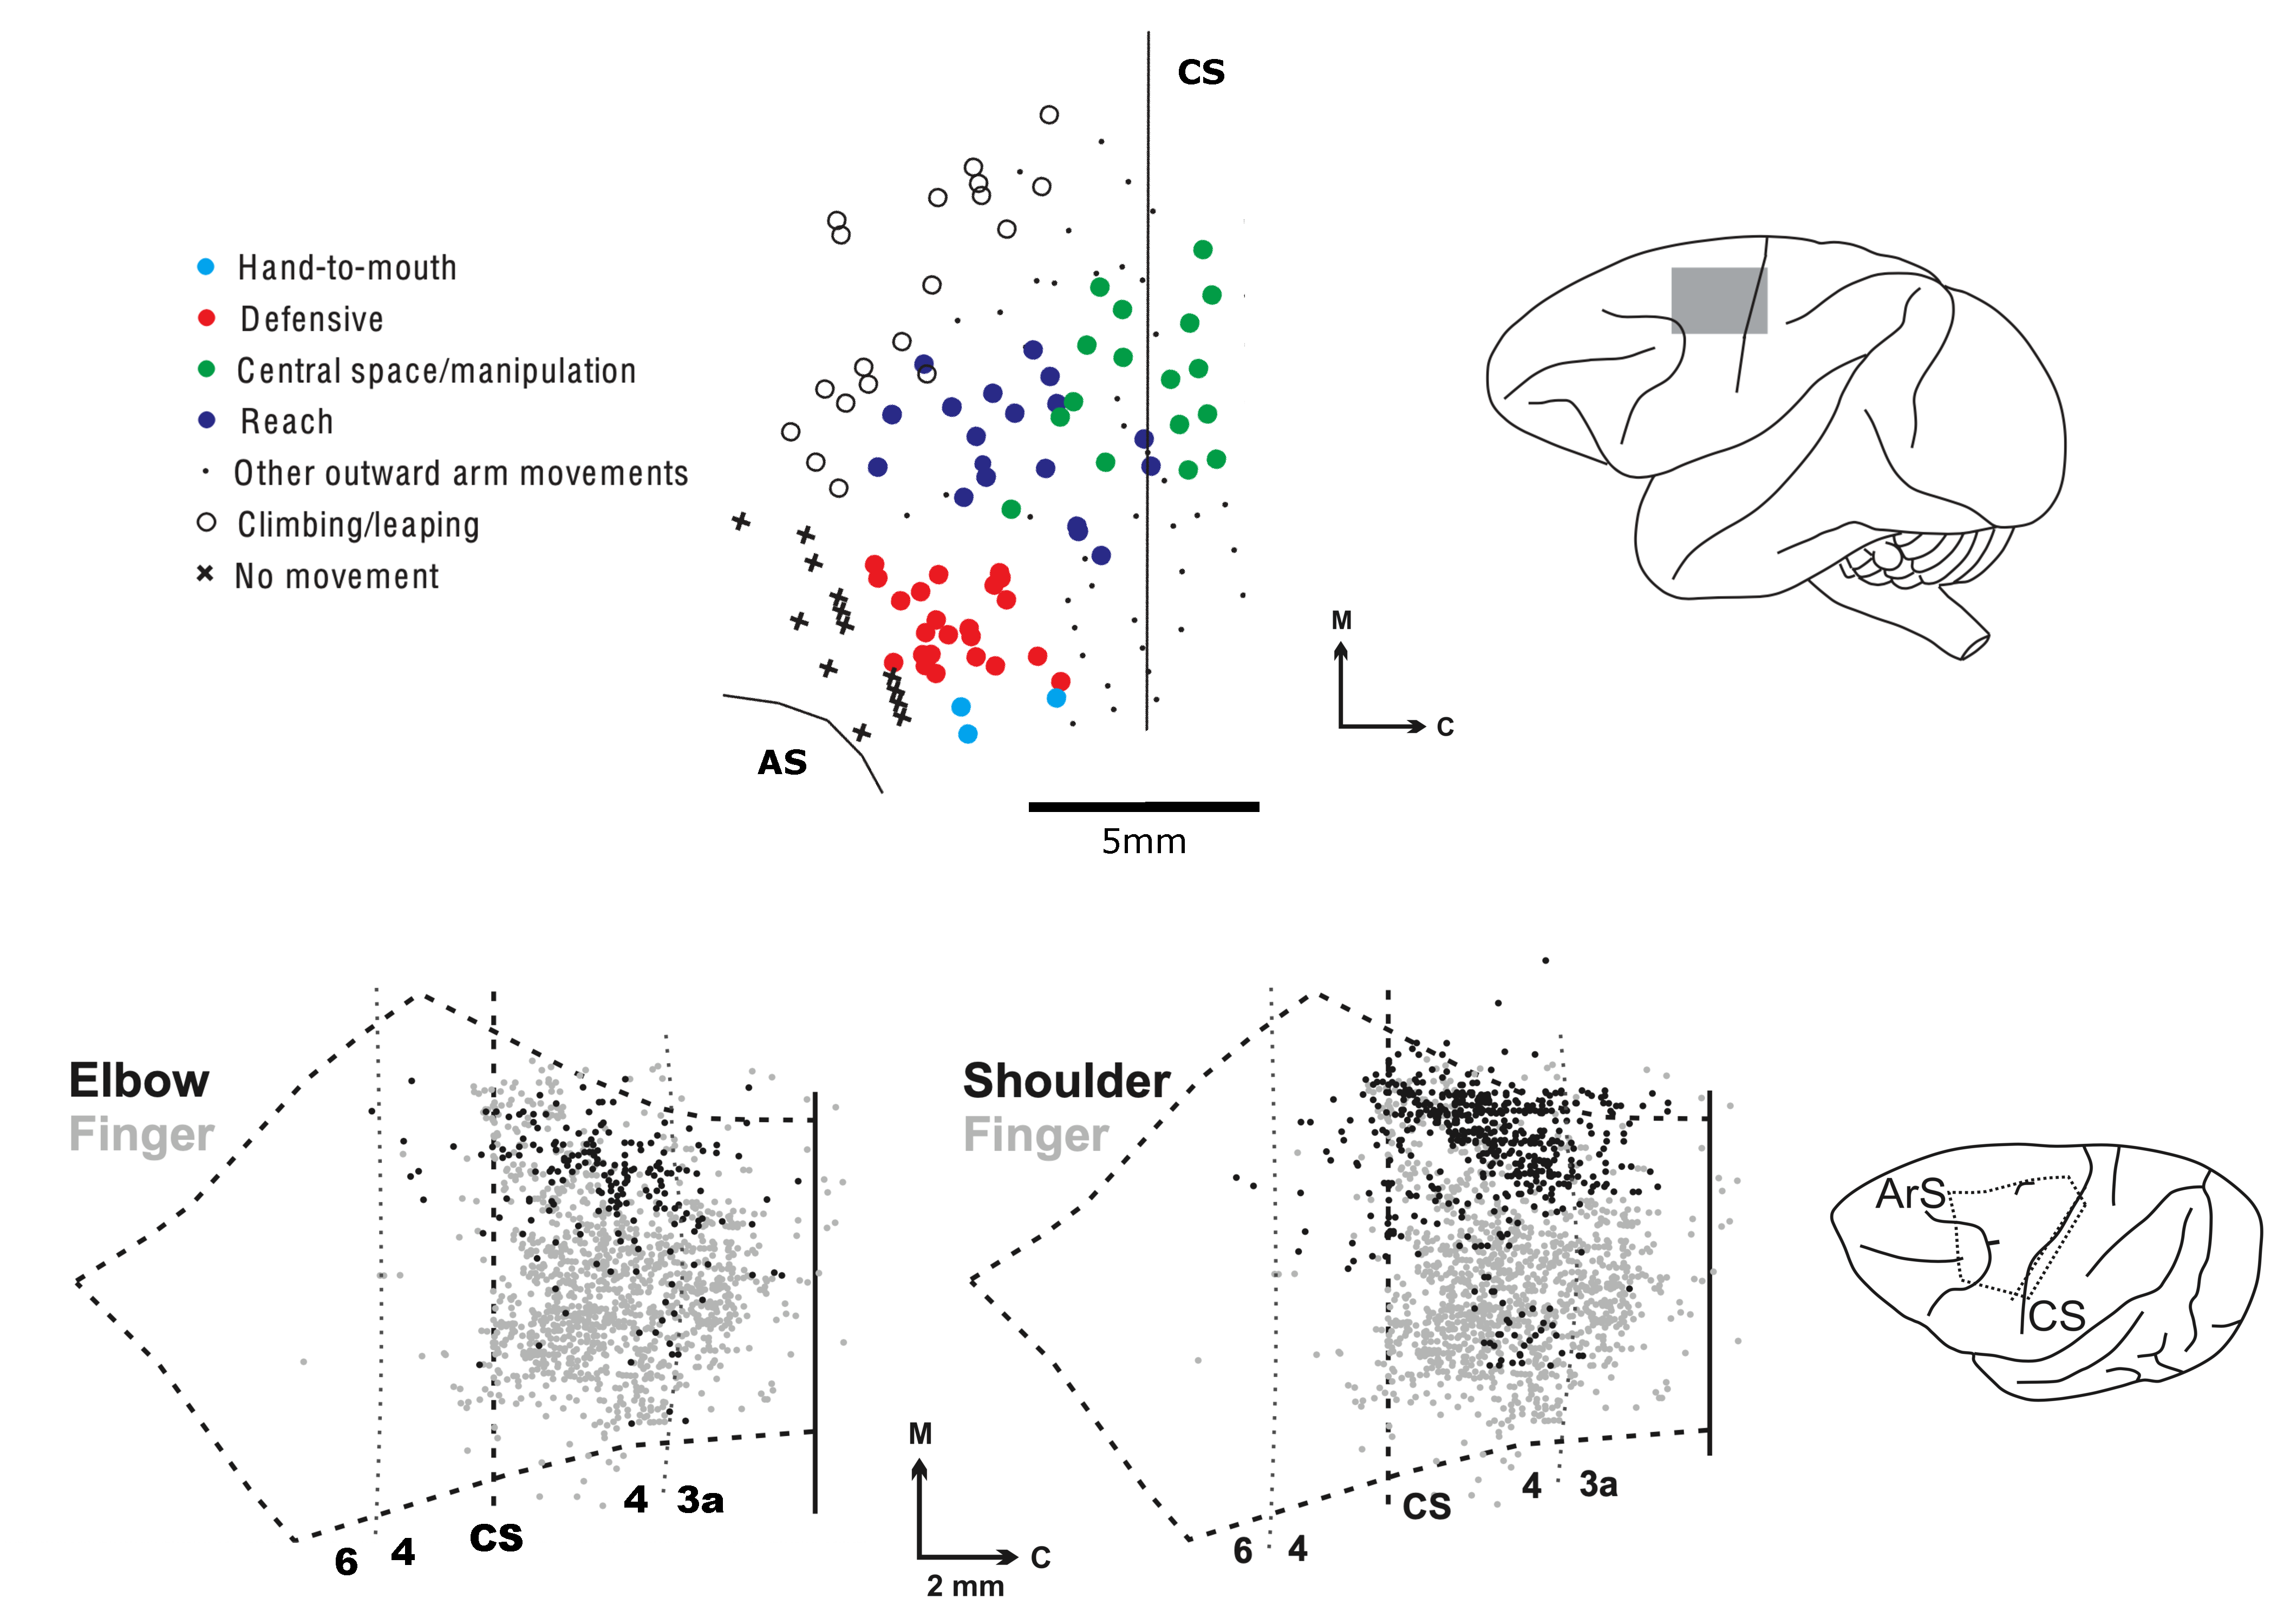
\includegraphics{images/physiology/strick_graziano/strick_graziano.pdf}
\caption{Similarities between electrical stimulation on behavorial
timescales and rabies tracing identification of CM cells. CM cells are
largely confined to the caudal half of M1, while this region tends to
evokes complex manipulatory movements when electrically stimulated. (Top
Left) Corticomotoneuronal (CM) cells traced using rabies from muscles of
the elbow and finger. (Top Right) CM cells traced using rabies from
muscles of the shoulder and finger. (Bottom) Complex movements evoked by
500ms electrical stimulation pulse trains. \emph{Adapted from Graziano
2005 and Rathelot 2009}}\label{fig:rathelot_graziano}
}
\end{figure}

\textbf{I added this on Friday:} \cref{fig:rathelot_graziano} depicts
the hierarchical nature of the motor system that enables its dexterity.
The motor system is tuned to produce varying levels of modularity, and
this is shown in Rasthelot's work at a structural level: CM cells
evolved to provide modifications to coarse, synergistic action. This is
reflectd in Graziano's work where, loosely, more dexterous behaviors are
produced when stimulation is applied to the caudal regions of motor
cortex. These dexterous behaviors are driven by a hierarchical stack of
cellular machinery, each level of which is modulated by estimated state,
goals, uncertainty, and value.

The movement machine reasons in the space of feedback control systems
and their ensuing trajectories. The phenomenal thing about the motor
system is that it is able to tune itself rapidly with both
high-dimensional sensory inputs and sparse reward
signals\textsuperscript{\protect\hyperlink{ref-bahlNeuralDynamicPoliciesfor2020}{39},\protect\hyperlink{ref-ijspeertDynamicalMovementPrimitives2013}{40}}.
This has some precedence in the literature and will be discussed further
in \cref{sec:theory}. This section has attempted to illustrate the
complexity of the motor control system specifically with regard to
dexterous control of the hand, with an eye toward experimental and
theoretical avenues for exploration. The goal is to build and test a
theoretical scheme for aspects of the compositional nature of the neural
hand controller.

\hypertarget{flexibilty-in-spinal-circuits}{%
\subsection{Flexibilty in Spinal
Circuits}\label{flexibilty-in-spinal-circuits}}

Renshaw cells -- synergist inhibition, maybe to synchronize synergistic
activations

\hypertarget{i-added-this-section-on-friday}{%
\subsubsection{I added this section on
Friday!**}\label{i-added-this-section-on-friday}}

Looking at rapid visuomotor responses, this work found that these
reflexive movement were modulated by the value of multiple goals, just
as in cognitive tasks. This supports the idea that there exists
flexibility at all ``levels'' of the hierarchy, all recieving similar
feedbacks and all similarly modulated by context:

\begin{quote}
If low-level sensorimotor circuits can contribute to value- based
decisions through continuous feedback control, rather than merely
executing the outcome of discrete action decisions taken in higher-order
brain areas, it would support for the hy- pothesis that value-based
decision algorithms are distributed throughout multiple levels of
sensorimotor and cognitive pro- cessing hierarchies (Hunt et al., 2014;
Hunt and Hayden, 2017). This notion differs from the traditional view
that decisions arise from a serial process with modular units for choice
evaluation, value comparison and action selection. According to the
alterna- tive view, the basis for decisions is mutual inhibition between
neural representations of alternative options, and these compu- tations
occur simultaneously in multiple brain areas along both motor and
abstract-value dimensions of tasks (Wang, 2012). Our current evidence
that value-based decisions can be implemented through sensorimotor
feedback control supports the alternative view, and the general notion
that behavior emerges via a distributed consensus between circuits
engaged nominally in decision and sensorimotor processes (Cisek,
2012).\textsuperscript{\protect\hyperlink{ref-carrollRapidVisuomotorResponses2019}{41}}
\end{quote}

\begin{quote}
When we move, the brain specifies a set of feedback control gains that
enable low-level motor areas not only to generate efficient and accurate
movement, but also to rapidly and adaptively respond to evolving sensory
information in a manner consistent with value-based
decision-making.\textsuperscript{\protect\hyperlink{ref-carrollRapidVisuomotorResponses2019}{41}}
\end{quote}

Spinal stretch reflexes may also be modulated by posture, like in
Graziano's work:

\begin{quote}
We found that changing the arm's orientation diametrically altered how
spinal reflexes in the elbow muscles were evoked, and in such a way that
were again efficiently scaled to the hand's distance from the target.
These findings demonstrate that spinal circuits can help efficiently
control the hand during dynamic reaching actions, and show that
efficient and flexible motor control is not exclusively dependent on
processing that occurs within supraspinal regions of the nervous
system.\textsuperscript{\protect\hyperlink{ref-weiler2020}{42}}
\end{quote}

This is supported by another paper:

\begin{quote}
Our results reveal complex goal-dependent modulation of fast feedback
responses in M1 that are present early enough to account for
goal-dependent stretch responses in arm
muscles\textsuperscript{\protect\hyperlink{ref-pruszynski2014}{43}}
\end{quote}

Feedback and internal dynamics play a role, and models reflect either
(in this model they forgo sensory feedback, which we see as integral to
modulating feedback control):

\begin{quote}
Sensory feedback takes at least 25 ms to influence cortical responses
and \textgreater50 ms to reflect the current goal. Thus, during this
\textasciitilde200-ms interval, the neural dynamics are not yet affected
by sensory feedback and should presumably be explained via internal
dynamics. This is true even of optimal feed- back control architectures,
which employ a dynamically varying control policy and internal
`efference-copy' recurrence to generate time-varying output patterns
before the arrival of feedback. Given the practical choice to use a
model without sensory feedback, we verified with additional simulations
that the solutions found by the model were robust to the addition of
reasonable forms of
feedback\textsuperscript{\protect\hyperlink{ref-sussillo2015}{44}}
\end{quote}

Andy has written that sensory and spinal systems work ``in parallel'',
but do we agree with this?

\begin{quote}
In terrestrial mammals, the rhythmic and coordinated leg movements
during locomotion are controlled by a combination of interconnected
neurons in the spinal cord, referred as to the central pattern
generator, and sensory feedback from the segmental somatosensory system
and supraspinal centers such as the vestibular system. How segmental
somatosensory and the vestibular systems work in parallel to enable
terrestrial mammals to locomote in a natural environment is still
relatively
obscure.\textsuperscript{\protect\hyperlink{ref-akayRelativeContributionProprioceptive2021}{45}}
\end{quote}

\hypertarget{the-heterarchical-motor-system}{%
\subsection{The Heterarchical Motor
System}\label{the-heterarchical-motor-system}}

This distributed view is crucial; a view that sensorimotor processing is
a, perhaps, ``complex hierarchy'', or even a heterarchy\ldots{}

\textsuperscript{\protect\hyperlink{ref-cohenRoleHeterarchicalControl1992}{46}}\textsuperscript{\protect\hyperlink{ref-huntDistributedHierarchicalRecurrent2017}{47}}
\textsuperscript{\protect\hyperlink{ref-huntHierarchicalCompetitionsSubserving2014}{48}}

This term was first used by McCulloch to describe the wat networks give
rise to multiple competing values:

\begin{quote}
Cir- cularities in preference instead of indicating inconsistencies,
actually demonstrate consistency of a higher order than had been dreamed
of in our philosophy. An organism possessed of this nervous system-- six
neurons-- is sufficiently endowed to be unpredictable from any theory
founded on a scale of values. It has a heterarchy of values, and is thus
internectively too rich to submit to a summum
bonum.\textsuperscript{\protect\hyperlink{ref-mccullochHeterarchyValuesDetermined1945}{49}}
\footnote{Supreme Good}
\end{quote}

He's saying that networks without a hierarchy of values, networks that
inherently loopy, give rise to ``unpredictability'', or perhaps
flexibility -- implies that if the system is optimizing, there is no
Supreme Good, but rather a composite Good comprised of component values.

Summum bonum is a Latin expression meaning the highest or ultimate good,
which was introduced by the Roman philosopher Cicero to denote the
fundamental principle on which some system of ethics is based --- that
is, the aim of actions, which, if consistently pursued, will lead to the
best possible life. (wiki)

used in social sciences to describe power relations between groups that
aren't strictly hierarchical, but exist in a more complex arrangement:

\begin{quote}
when a given production mechanism is regulated by multiple control
mechanisms without these control mechanisms being themselves sub- sumed
under a higher-level controller. To the degree one can distinguish
levels of control, there may be more control- lers at higher levels than
at lower
levels\textsuperscript{\protect\hyperlink{ref-crumleyHeterarchyAnalysisComplex2008}{50}}
\end{quote}

\begin{quote}
The addition of the term heterarchy to the vocabulary of power relations
reminds us that forms of order exist that are not exclusively
hierarchical and that interactive elements in complex systems need not
be permanently ranked relative to one
another.\textsuperscript{\protect\hyperlink{ref-crumleyHeterarchyAnalysisComplex2008}{50}}
\end{quote}

\begin{quote}
many structures, both biological and social, are not organized
hierarchically. There is nothing intrinsically hierarchical about an oak
tree or a symphony, yet each has undeniable structure and constitutes an
orderly repre- sentation of the relations among elements. Nonetheless,
few terms identify other kinds of order. Hier- archy---inasmuch as it is
often a reductionist metaphor for order---has disproportionately
influenced theory building in both social and natural scientific
contexts.\textsuperscript{\protect\hyperlink{ref-crumleyHeterarchyAnalysisComplex2008}{50}}
\end{quote}

\begin{quote}
control hierarchy: decisions at higher levels affect the operation of
lower
levels.\textsuperscript{\protect\hyperlink{ref-crumleyHeterarchyAnalysisComplex2008}{50}}
\end{quote}

is this really a good definition? i suppose it's something about the
agency of the decisionmaking, it's more about control -- does the
upstream control only the downstream?

in philosophy: \textgreater{} when a given production mechanism is
regulated by multiple control mechanisms without these control
mechanisms being themselves sub- sumed under a higher-level controller.
To the degree one can distinguish levels of control, there may be more
control- lers at higher levels than at lower
levels\textsuperscript{\protect\hyperlink{ref-bechtelGroundingCognitionHeterarchical2021}{51}}

\begin{quote}
\ldots the formation of a voluntary movement is much more complicated.
To think that a voluntary action is formed in the narrow field of the
motor cortex would be a mistake similar to an assumption that all the
goods exported through a terminal are produced in the terminal. The
system of cortical zones participating in the creation of a voluntary
movement includes a complex of subcortical and cortical zones, each
playing a highly specific role in the whole functional system.
\end{quote}

shift in vernacular can be a shift in knowledge point of science is to
describe the world concretely, so our words using to do this description
matter

\hypertarget{sec:experiment}{%
\section{Background Experimental Methods}\label{sec:experiment}}

\begin{itemize}
\tightlist
\item
  what are the most important concepts / results that inform our
  experiments?
\item
  What do we think we know from experiments about motor control? motor
  adaptation? motor learning?
\end{itemize}

\hypertarget{control}{%
\subsection{Control}\label{control}}

Is LQR (as it's claimed to be) a reasonable model for feedback control
and error reduction + variability prediction for dimensionality
reduction-based motor interface

(task reads out from D muscles, find modes of that data; do PCA to get K
\textless{} D dimensions, controller only responds to motion in those K
directions)---does behavior + motor activity follow LQR? this question
has already been asked, but it hasn't been asked for this kind of
high-to-low dim mapping. It's been asked in tasks where muscles haven't
been directly in control (Bolero 2009). Todorov: do a task, look at
muscle signal. Muscles that aren't necessary for task have higher
variability b/c they're not being optimized for task (but does't
introduce perturbations). Also see Loeb (2012) for a negative result
saying that muscle coordination is habitual rather than optimal, but it
has issues (low \# muscles). Can we replicate previous reaching
optimality results in our set-up? What's unique about our set-up is the
PCA/dimensionality reduction in muscle activity space. This is important
because you can create arbitrary muscle-cursor mappings, so you have to
learn a new skill/mapping. This is different than perturbing a
fundamental movement and forcing adaptation, which is what has been
previously done. For our task, the participants actually have to learn a
new task/mapping, rather than just do what they already know and be
robust to perturbations. We test the LQR hypothesis once they've learned
the task, because LQR isn't a learning theory, it's a theory about
optimal control. We can see if, once people learn a new skill, their
behavior is optimal wrt LQR theory. If we establish this, then we can
think about how this LQR model is actually learned (enter RL).

Our results are consistent with a recently described model in which an
optimal feedback control policy is calculated independently for each
potential target and a weighted average of these policies (that is,
feedback gains) is computed at each point in time based on the relative
desirability of each target50. Notably, this model, which pre-dicts
averaging of feedback gains, can also account for spatial (that is,
trajectory) averaging in go-before-you-know tasks. We submit that our
result showing feedback gain averaging, coupled with previous work
demonstrating trajectory averaging, provides strong support for the
compelling idea that the CNS, under cases of target uncertainty, encodes
in parallel multiple motor plans, along with their associated control
policies, for competing action options. (Wolpert Nature 2018 competing
control policies)

Nashed 2014 -- short-latency R1 and long-latency R2 responses (60ms;
45--75ms; 75--105 ms) stretch responses R1 show dexterity (Andrew Pru
2019,2020) in holding and in reaching

\hypertarget{adaptation-of-reaching}{%
\subsubsection{Adaptation of Reaching}\label{adaptation-of-reaching}}

\begin{itemize}
\tightlist
\item
  prisms
\item
  rotations
\item
  forcefield
\item
  nothing -- van Beers variability
\end{itemize}

\begin{quote}
The vast majority of research in motor learning studies this capacity
through adaptation para- digms in which a systematic perturbation is
introduced to disrupt a well-practiced behavior, such as point-to-point
reaching.\textsuperscript{\protect\hyperlink{ref-adrianTheoreticalModelsMotor2012}{52}}
\end{quote}

\begin{itemize}
\tightlist
\item
  classic reaching adaptation --\textgreater{} this is a different goal

  \begin{itemize}
  \tightlist
  \item
    shadmehr
  \item
    krakauer
  \end{itemize}
\item
  unperturbed movements

  \begin{itemize}
  \tightlist
  \item
    van beers
  \end{itemize}
\end{itemize}

\textsuperscript{\protect\hyperlink{ref-Krakauer2019}{53},\protect\hyperlink{ref-Shadmehr2008}{54}}

There exist a handful of prior studies mapping EMG activity and finger
joint angles directly to virtual stimuli, though few are focused on the
learning process and none have the input dimensionality we aim to
achieve in work proposed here.

\textsuperscript{\protect\hyperlink{ref-vanbeersRandomWalkMotor2013}{57}}

\hypertarget{arbitrary-visuomotor-mappings}{%
\subsubsection{Arbitrary Visuomotor
Mappings}\label{arbitrary-visuomotor-mappings}}

\textsuperscript{\protect\hyperlink{ref-Mussa-IvaldiSensoryMotorRemapping2011}{58}}

There are several studies using non-EMG-driven sensorimotor mappings to
study human motor control and learning.

\begin{itemize}
\tightlist
\item
  Remapping Hand Movements in a Novel Geometrical Environment
  https://www.ncbi.nlm.nih.gov/pubmed/16148276
\end{itemize}

\textsuperscript{\protect\hyperlink{ref-MosierRemappingHandMovements2005}{59}}

vocoder machine bell labs

Hinton, Fells

palsy study

takehome: humans are really good at learning tasks like these,
especially with their hands. this type of dexterity is specific to
primates if not humans. let's use this ability to understand and try to
model how this learning process unfolds.

\textbf{\emph{What does this give us that a force-field reaching task
can't?}}

\textsuperscript{\protect\hyperlink{ref-nazarpourFlexibleCorticalControl2012}{60}}

\hypertarget{skill-learning-tasks}{%
\subsubsection{Skill Learning Tasks}\label{skill-learning-tasks}}

\begin{itemize}
\tightlist
\item
  skill learning tasks

  \begin{itemize}
  \tightlist
  \item
    ball and cup
  \item
    dart throwing tasks
  \end{itemize}
\end{itemize}

\hypertarget{learning-in-cortical-interfaces}{%
\subsubsection{Learning in Cortical
Interfaces}\label{learning-in-cortical-interfaces}}

\begin{itemize}
\item
  cortical BMI work

  \begin{itemize}
  \tightlist
  \item
    Batista papers, lee miller papers
  \end{itemize}
\item
  speech learning -- analogy to speech
\item
  bird vocal learning
\item
  we're doing the same experiment, at the muscle level
\item
  try to convince why this is useful, but not too hard
\end{itemize}

\hypertarget{properties-of-electromyographic-signals}{%
\subsection{Properties of Electromyographic
Signals}\label{properties-of-electromyographic-signals}}

\begin{itemize}
\tightlist
\item
  not actually gaussian, but
  super-gaussian\textsuperscript{\protect\hyperlink{ref-nazarpourNoteProbabilityDistribution2013}{61}}
\item
  some work using bayesian filtering methods to infer the signal
  envelope\textsuperscript{\protect\hyperlink{ref-sangerBayesianFilteringMyoelectric2007}{62}}
\item
  Farina paper on EMG as convolution
\end{itemize}

A window of EMG of length \(T\) samples can be modeled like

\[
\mathbf{z} = \sum_t^T \mathbf{h} * \mathbf{s}
\]

where \(\mathbf{h}\) is a motor unit activation template, which itself
is a particular neural spike waveform, and \(\mathbf{s}\) is the
incidence of a spike, which might be modeled as a point process.

\begin{quote}
EMG records were rectified, smoothed and averaged before further
analysis.\textsuperscript{\protect\hyperlink{ref-churchlandNeuralPopulationDynamics2012a}{63}}
\end{quote}

\begin{quote}
EMG activity was recorded using hook-wire electrodes (44 gauge with a 27
gauge cannula; Nicolet Biomedical, Madison, WI) placed in the muscle for
the duration of single recording sessions. {[}\ldots{]} Electrode
voltages were amplified, bandpass filtered (150--500 Hz, four pole, 24
db/octave), sampled at 1000 Hz, and digitized. Off-line, raw traces were
differentiated (to remove any remaining baseline), rectified, smoothed
with a Gaussian (SD of 15 ms) and
averaged.\textsuperscript{\protect\hyperlink{ref-churchlandNeuralVariabilityPremotor2006}{64}}
\end{quote}

inter-subject variability is high, but seems to show individual
strategies for
movement\textsuperscript{\protect\hyperlink{ref-crouzierIndividualDifferencesDistribution2019}{65}}

The surface EMG signal can be modeled as the convolution of

Can muscle coordination be precisely studied by surface
electromyography?\textsuperscript{\protect\hyperlink{ref-Hug2011}{66}}

This requires first mapping the intrinsic available dynamics of the hand
per user.

\hypertarget{skill-learning-in-myolectric-interfaces}{%
\subsubsection{Skill Learning in Myolectric
Interfaces}\label{skill-learning-in-myolectric-interfaces}}

``performance levels and rates of improvement were significantly higher
for intrinsic hand muscles relative to muscles of the
forearm.''\textsuperscript{\protect\hyperlink{ref-Dyson2018}{67}}

\hypertarget{berger-et-al.-2013}{%
\subsubsection{Berger et al.~2013}\label{berger-et-al.-2013}}

\textsuperscript{\protect\hyperlink{ref-BergerDifferencesInAdaptationRates2013a}{68}}

Berger et al.'s preprocessing - lowpassed butterworth at 5Hz -
normalized to MVC calibration - periodic baseline noise substraction -
choosing synergies by uniformity in force direction (pretty arbitrary)

Using EMG in a learning experiment is not unheard of. Berger et al.~2013
use EMG with 13 muscles to test whether learning new synergy
combinations for a task is more difficult that recombining existing
synergies@Berger2013a. As we would expect, learning new synergy
combinations is more difficult. I would argue that the demand in their
``incompatible virtual surgeries'' is too strict, that we need to more
carefully design synergy perturbations to develop a model of learning in
such a task.

Berger et al.~fit a muscle-space to force-space mapping \(H\) using a
force-driven calibration task, and a synergy-space to muscle-space
mapping \(W\) using NMF.

\begin{align*}
    f &= Hm \\
    m &= Wc
\end{align*}

\(\dim(m)=M\) muscles, \(\dim(c)=N\) synergies, and \(\dim(f)=D\)
dimensions of task space where \(M>N>D\). Because \(H\) and \(W\) are
rectangular, they have at most rank \(D\) and \(N\), and we constrain
these matrices to be full rank. There are three key subspaces: the
nullspace of \(H\) mapping muscle activations to 0, the column space or
range of \(W\) mapping synergy activations to muscle activations, and
the common subspace between these two. That is, there are synergy
activations which generate muscle activations which lie in the null
space of \(H\). The paper uses this fact to develop mappings that
specifically rotate muscle activations produced by synergies into the
null space of \(H\) which were not there prior to rotation. The
dimensionalities of these subspaces are defined:

\begin{align*}
\dim(\mathrm{null}(H)) &= M - D && \text{muscle vectors $\rightarrow$ 0} \\
\dim(\mathrm{col}(W)) &= N && \text{synergy activations $\rightarrow$ muscle subspace}\\
\dim(\mathrm{null}(H)\cap\mathrm{col}(W)) &= N - D && \text{synergy activations $\rightarrow$ 0} \\
\end{align*}

In the paper, the authors find an orthonormal basis \(W_o\) for the
range (column space) of the synergy weight matrix \(W\) (presumably
using a QR factorization) and find the nullspace \(H_{null}\) of \(H\).
These computations are done presumably through QR factorizations (an
orthonormal basis multiplied by a rotation and scaling) by finding \(Q\)
in the first case and finding the latter \(M-D\) columns \(Q_2\) of
\(Q = [Q_1 \, Q_2]\) which are \(H_{null}\) in the second case:

\begin{align*}
    W &= Q_W^{M\times M}R_W^{M\times N} \\
      &= \left[Q_{W,1}^{M\times N}\,Q_{W,2}^{M\times M-N}\right]\begin{bmatrix}R_{W,1} \\ 0 \end{bmatrix} \\
    W_o &= Q_{W,1}^{M\times N} \\
    W_o^T &= Q_{W,1}^{T, N\times M} \\
    H^T_{M\times D} &= Q_H^{M\times M}R_H = \left[Q_{H,1}^{M\times D}\,Q_{H,2}^{M\times M-D}\right]\begin{bmatrix}R_{H,1} \\ 0 \end{bmatrix} \\
    H^T_{null} &= Q_{H,2}^{M\times M-D}
\end{align*}

To find each of the three subspace, we take the SVD of the composition
\(W^TH^T\)

\begin{align*}
    W_o^TH^T_{null} &= Q_{W,1}^{T, N\times M} Q_{H,2}^{M\times M-D} \\
    &= Q^T_WQ_H && \dim(N \times M-D) \\
    &= U_{N\times N}\Sigma_{N \times M-D} V^T_{M-D\times M-D} \\
    H^T_{null}V &= W_oU\Sigma
\end{align*}

Now we can pick out the three subspaces using the SVD

\begin{align*}
    W_c &= W_oU[1:N-D] && \text{synergy activations $\rightarrow$ muscle activations in task null space}\\
    H_c &= H_{null}[1:N-D] && \text{synergetic muscle activations $\rightarrow$ 0} \\
    W_{nc} &= W_oU[N-D+1:N] && \text{synergy activations $\rightarrow$ nonzero muscle activations}\\
    H_{nc} &= H_{null}V[N-D+1:M-D && \text{non-synergetic muscle activations $\rightarrow$ 0} \\
\end{align*}

To construct new mappings, the authors construct rotations to alter
muscle activation vectors by rotating them from \(W_nc\) and remaining
in \(W_nc\) and from \(W_nc\) into \(H_nc\). In the first case this
alters the mapping by changing the effective muscle activations produced
by the existing (learned) synergetic actions. That is, muscle
activations putatively produced by synergetic action will be altered to
produce different forces in task space (compatible rotations). In the
second case, muscle activations putatively produced by existing
synergetic action (via W) will be mapped into the null space of \(H\)
and produce zero force in task space (incompatible rotations).

A key critique of this paper is that such a transformation is too harsh.
The compatible rotation allows you to recombine the same muscle
patterns, the incompatible doesn't allow you to use existing
coactivation patterns at all. The authors do see new synergies emerging
even after their training session, consisting of:

\begin{itemize}
\tightlist
\item
  16 trials of maximum voluntary contraction in 8 directions
  (calibration)
\item
  72 trials using force control (calibration)
\item
  24 trials familiarization
\item
  144 trials baseline
\item
  288 trials surgery
\item
  144 trials washout
\item
  144 trials baseline
\end{itemize}

After 288 trials subjects aren't able to complete the task for some
movement directions.

\hypertarget{nazarpour-2012-j.neuro}{%
\subsubsection{Nazarpour 2012 J.Neuro}\label{nazarpour-2012-j.neuro}}

\textsuperscript{\protect\hyperlink{ref-nazarpourFlexibleCorticalControl2012}{60}}

x Flexible Cortical Control of Task-Specific Muscle Synergies
https://www.jneurosci.org/content/32/36/12349

Fig. 4A -- cursor controlled muscles begin to dissociate from non cursor
controlled muscles.

Feedforward processing to muscle fields / tunings in the presence of
signal dependent noise

Feedback processing based on visual errors

\hypertarget{radhakrishnan-2008}{%
\subsubsection{Radhakrishnan 2008}\label{radhakrishnan-2008}}

\textsuperscript{\protect\hyperlink{ref-radhakrishnanLearningNovelMyoelectricControlled2008}{69}}

x Learning a Novel Myoelectric-Controlled Interface Task ---
Radhakrishnan, 2008
https://www.ncbi.nlm.nih.gov/pmc/articles/PMC2576223/

proprioception is not required to learn nonintuitive MCI mappings

several hundred trials subjects learned pointing with six muscles

prism adaption requires active movement; efference copy implicated if
proprioception doesn't seem to be required

control models Fig 10

\hypertarget{de-rugy-2012---habitual-not-optimal}{%
\subsubsection{de Rugy 2012 - Habitual not
Optimal}\label{de-rugy-2012---habitual-not-optimal}}

\textsuperscript{\protect\hyperlink{ref-derugyMuscleCoordinationHabitual2012}{70}}

just because it's harder to adapt to incompatible surgeries doesn't mean
that there are fixed synergies, it just means there are multiple
timescales of adaptation available in the neural control hierarchy --
diversity in the neural controller depending on context

learning inverse model may be separate from learning to optimize
trajectories on top of that model -- some type of ``fine tuning''

skill acquisition (slow, constructing novel synergies) vs.~motor
adaptation (less slow, adapting existing synergy activations)

It's a good test, but it pushes the optimal control framework too hard?
perhaps we need a model for what ``good enough'' is? If we penalize
moving to a new controller from a previously optimized movement, the
findings make sense. An optimal control model would predict the exactly
optimal coordination patterns for the new scenario, it wouldn't say
anything about adaptation from an old solution to a new one. This is why
we need to develop a model of adaptation that formalizes this scenario
not of kinematic perturbations (noise during movement), but to a drastic
change in the plant itself (e.g.~muscle failure).

\hypertarget{mussa-ivaldi-2019}{%
\subsubsection{Mussa-Ivaldi 2019}\label{mussa-ivaldi-2019}}

\begin{quote}
Earlier theoretical work by Jordan and Rumelhart {[}14{]} considered how
the learning of actions can be viewed as the concurrent learning of for-
ward and inverse models of actions. \textbf{They introduced the concept
of distal learning, where the learner has to find a mapping from desired
outcomes to actions in order to achieve a desired outcome. To do so, the
subject begins by forming a predictive forward model of the
transformation from actions to distal outcomes. Such transformations are
often not known a priori, thus the forward model must generally be
learned by exploring the outcomes associated with particular choices of
action. Once the forward model has been at least partially learned, it
can be used to guide the learning of an inverse model that predicts the
action needed to achieve the distal outcome.} Mussa-Ivaldi2019
\end{quote}

\begin{quote}
Our findings are consistent with the hypothesis that learning proceeds
through the concurrent evolution of cou- pled forward and inverse models
of the body-to-object mapping established by the BoMI. Mussa-Ivaldi2019
\end{quote}

\begin{quote}
Not being square, the matrix H does not have a unique inverse. But there
exist infinite ``right inverses'' that combined with H yield the K x K
identity matrix in the task space of exter- nal control signals. Each
such right inverse transforms a desired position of the controlled
object into one particular set of values for the body signals. We
consider users to be competent when they are able to move their body
successfully in response to a presented target for the controlled
object. Mathematically, we consider this as finding one right inverse G
of the map- ping H, out of a multitude of possible and equally valid
choices. Mussa-Ivaldi2019
\end{quote}

Gradient learning of a forward and inverse model (mapping):

\begin{align*}
    \hat{H}_{n+1} &= \hat{H}_n + \epsilon(p_n - H_nq_n)q_n^T  \\
    G_{n+1} &= G_n - \eta\hat{H}_n^Te_nu_n^T \\
    e_n &= p_n - u_n
\end{align*}

\begin{quote}
The comparison between model predictions and actual data in Fig 3
indicates that our proposed model of learning is sufficient to explain
the data. However, the mechanism we propose is not necessary; we cannot
rule out other possibilities, such as reinforcement learning.
{[}\ldots{]} This agreement between model and experimental results does
not exclude the possibility of alternative learning mechanisms, such as
a direct learning of the inverse model {[}24{]} or the use of
reinforcement learning {[}25{]} to acquire an action policy that would
play the role of the inverse model. Mussa-Ivaldi2019
\end{quote}

How do we break a simple gradient model? On a task that is more
difficult? will learning take longer? - savings phenomenon -

\begin{quote}
Although the interface forward map is linear (Methods, Eq (5)), this is
a many-to-one map admitting a multitude of inverses. This ``redundancy''
opens the possibility of successful linear and nonlinear inverse maps.
Redundancy also leads to an important consideration about gradient
descent learning. The reaching error surface in the space of the inverse
model elements does not have a unique minimum, but a continuously
connected set of minima corresponding to the null space of the forward
map. In the metaphor of a skier descending from a mountain following the
gradient, this space of equivalent inverse models corresponds to a flat
elongated valley at the bot- tom of the mountain. Anywhere along the
valley is a valid end to the ride, as it corresponds to a valid inverse
model. The inverse model on which the steepest descent ends depends on
the initial conditions, as predicted by the dynamical model (see Fig
3b--evolution of the norm of the inverse model error), as well as on the
realization of the noise employed in any given simulation of the
learning model.
\end{quote}

\begin{quote}
Although the two-dimensional subspace formed by the first two PCs
captured a large fraction of the total variance of body motions, it did
not necessarily reflect the natural up-down/left-right orientation of
the display monitor. Therefore, following calibration and PC extraction,
there was a customization phase in which users were allowed to set the
origin, orientation, and scaling of the coordinates in task space, based
on their preference.
\end{quote}

Subjects have prior knowledge of their directions in task space?

x 90\% isn't enough -- Follow-up on the previous paper -- critiques
``direct evidence'' https://www.biorxiv.org/content/10.1101/634758v1

\begin{itemize}
\tightlist
\item
  Structured variability of muscle activations supports the minimal
  intervention principle of motor control
  https://www.ncbi.nlm.nih.gov/pubmed/19369362
\end{itemize}

\hypertarget{sec:experiment}{%
\section{Experimental Contributions}\label{sec:experiment}}

\begin{itemize}
\tightlist
\item
  shape of the data
\item
  structure of variability in the EMG compared to the structure of
  variability in the behavior?
\end{itemize}

\begin{quote}
we know how to design and interpret experiments that involve many
repetitions of the same movement however there is limited role for
online optimization in that context. instead we need experiments where
subjects are required to come up with new movements all the time. how
can we get experimenters to do such experiments? show cool movies of
robots doing cool things,and hopefully get the experimenters excited.
(todorov online optimization slides)
\end{quote}

\hypertarget{experimental-setup}{%
\subsection{Experimental Setup}\label{experimental-setup}}

My setup records EMG from the forearm.

The goal of the project's first phase is to develop a high-dimensional
surface EMG recording rig to generate datasets with high signal-to-noise
ratio and dense coverage over superficial muscles of the arm and hand.
The first question of this phase is: what are the limitations of a
closed-loop myocontrol experiment, and how can such constraints be
avoided or leveraged? To answer this question we will develop a signal
processing pipeline and diagnostics suite to identify constraints in the
setup and aim to overcome, as much as possible, the limitations inherent
in surface EMG recording such as muscle crosstalk and rigorous electrode
placement.

The concept of the experimental setup is shown in Figure 1, where 64
monopolar electrodes are attached to a subject's arm and hand to record
muscle activity. The arm and hand are kinematically constrained in a
custom fixture and motor activity is recorded during isometric muscle
contractions at levels less than 20\% maximum voluntary contraction to
lessen the risk of involuntary co-contractions. The setup circumvents
the limb biomechanics by mapping muscle output directly to virtual
stimuli shown on a computer monitor. Additionally, our study focuses on
low-force, isometric contractions to avoid complications due to
artifacts in dynamic, high- force movements.

We chose 64 channels in order to have at least two electrodes per muscle
implicated in control of the hand in the event that we require
differential recording. This choice limits our analysis to the motor
pool level. If our questions require recording at the motor unit level,
we will need to move to a higher channel count system. Literature in
this field typically use a much lower number of channels. We believe
that using 64 electrodes will help develop a more complete picture of
the superficial muscle activity of the arm and hand across learning. A
diagram of muscles relevant to thee control of the hand and wrist is
shown in Figure 2 on page 4. We are not aware of a rigorous study
testing which muscles of the arm and hand can be accurately captured
using surface EMG.

\begin{fignos:no-prefix-figure-caption}

\begin{figure}
\centering
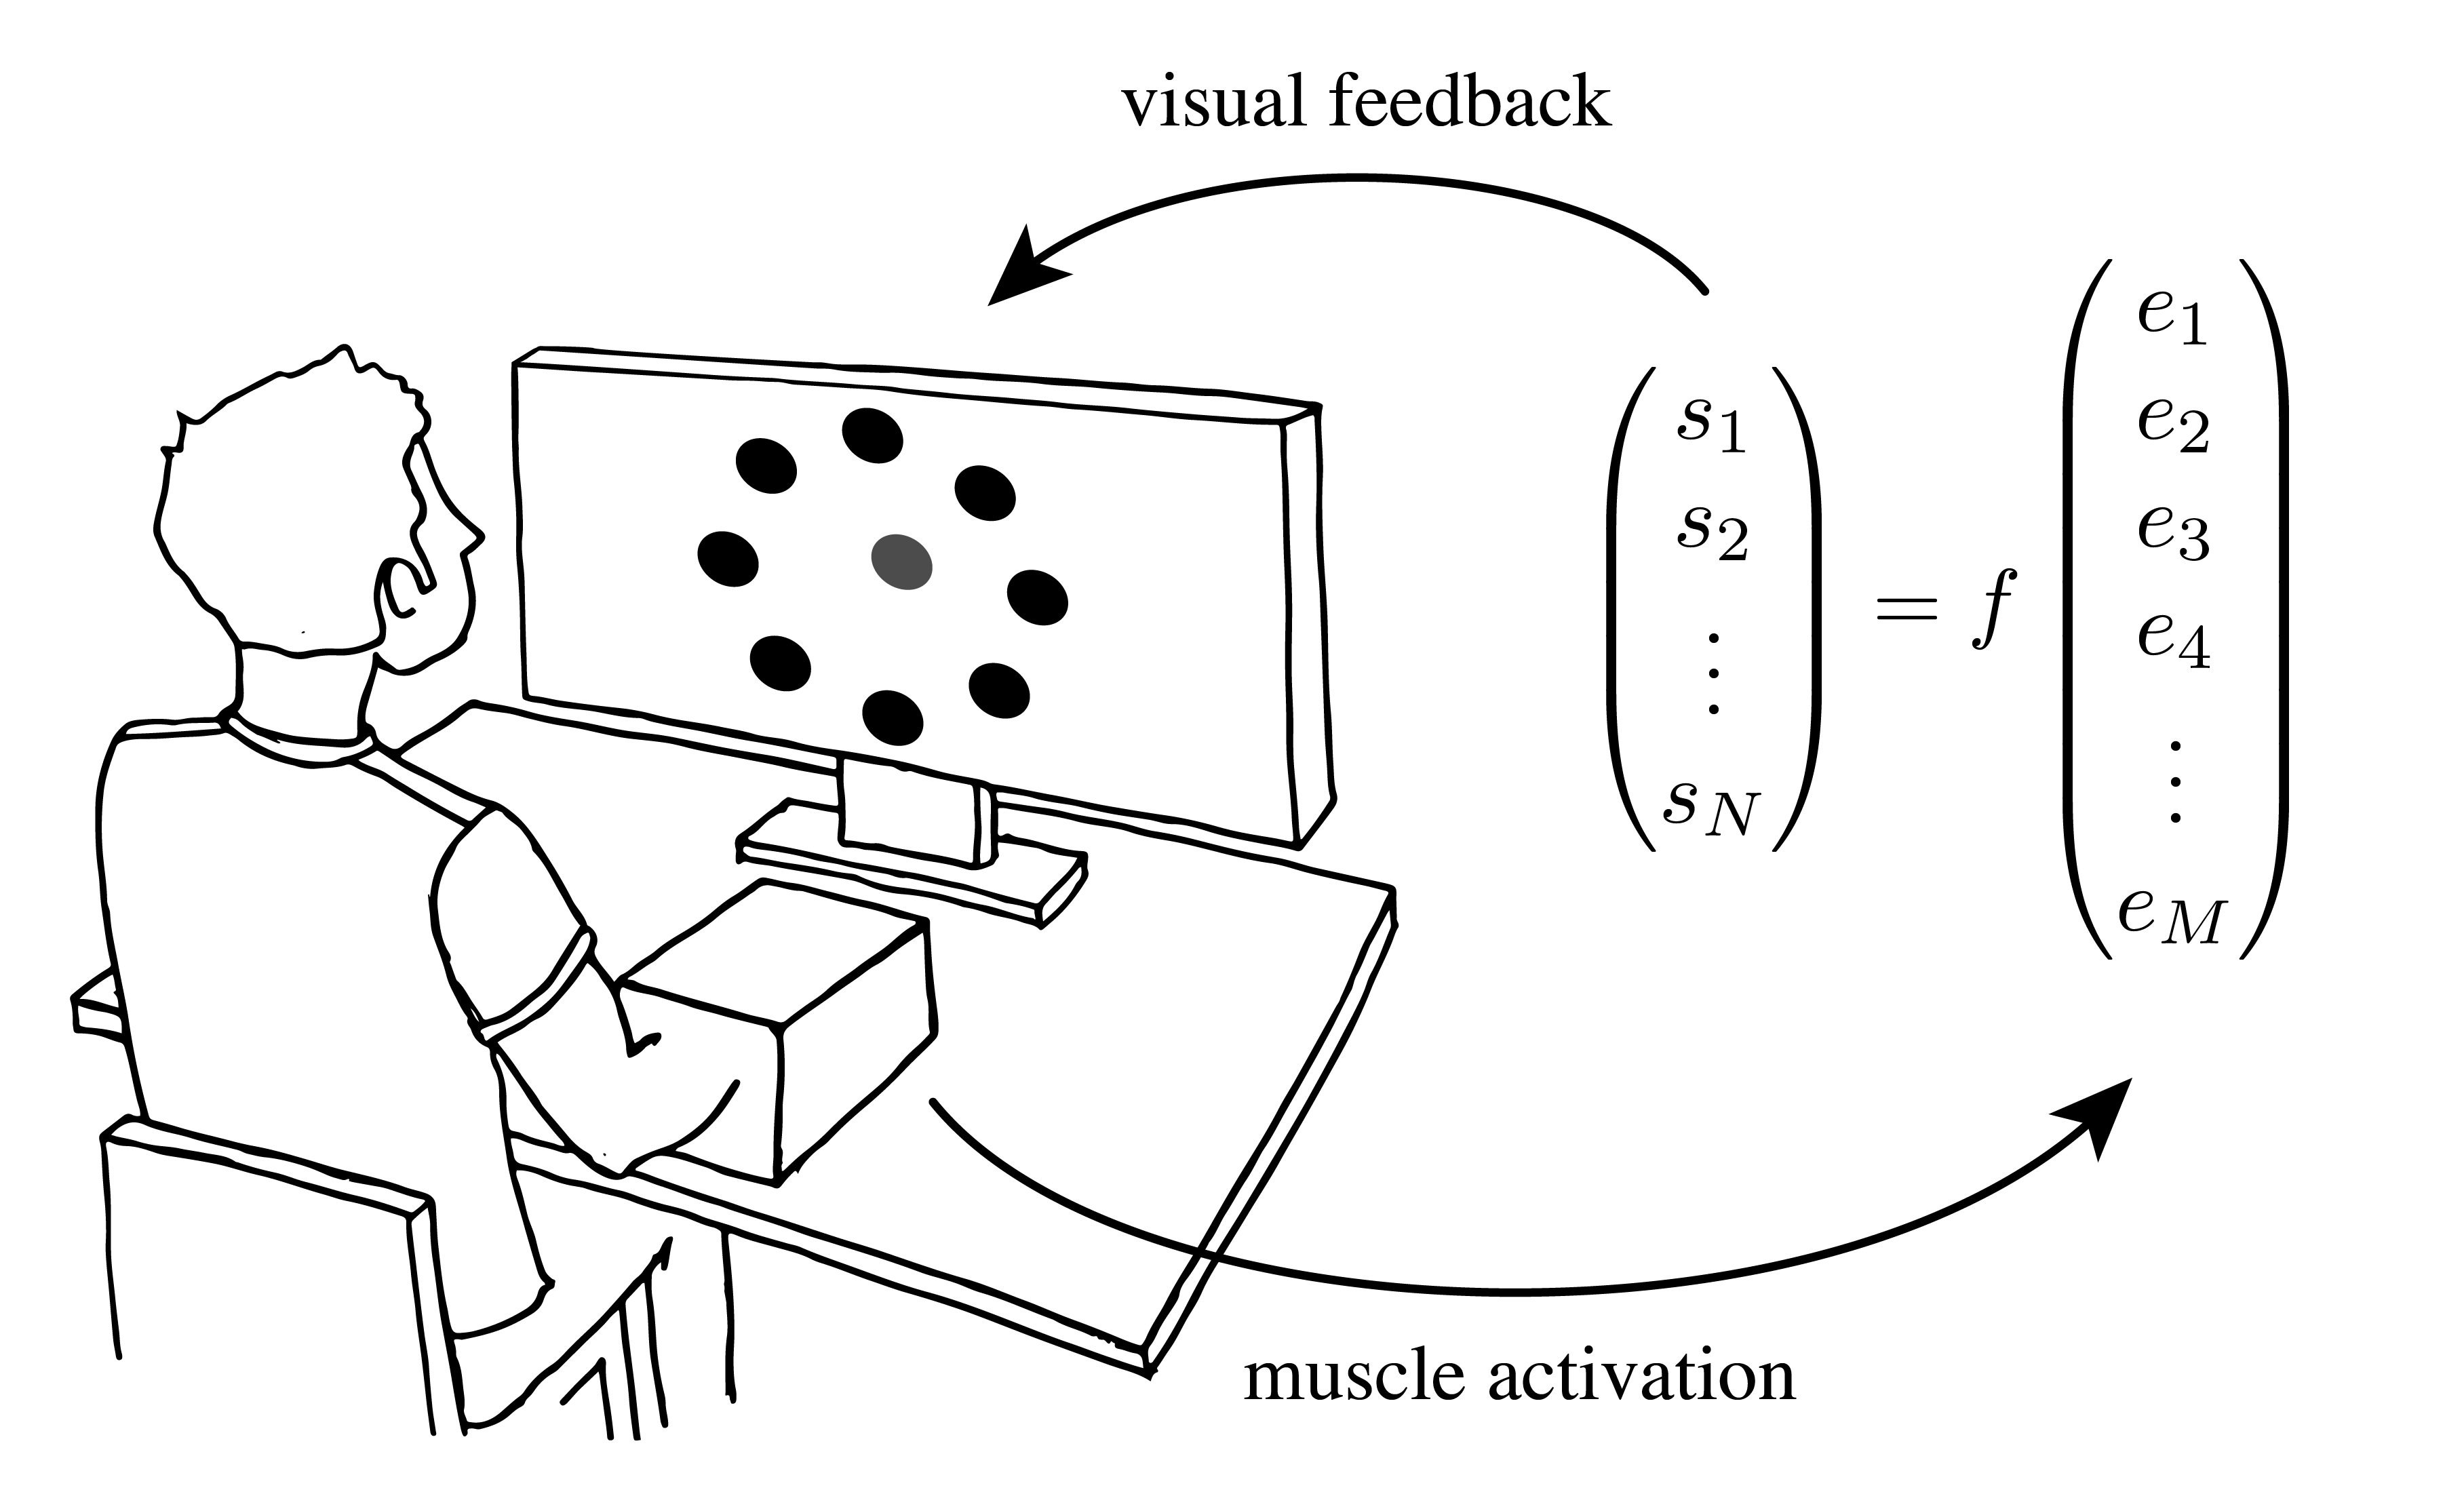
\includegraphics{images/graphics/desk.png}
\caption{Sketch of the experimental concept}
\end{figure}

\end{fignos:no-prefix-figure-caption}

We aim to extend this prior work using learning algorithms that take
into account time- varying dynamics of the signal in addition to common
tools like components analysis and matrix factorization. This analysis
will help generate an understanding of intersubject, intersession, and
intertask variability. Both an analysis of dynamic correlations and a
validation of dimensionality using EMG would be a novel contribution to
the literature.

We anticipate that quantifying electrode placement and calibrating
across sessions will be a major challenge. We aim to develop a
mechanical fixture for recording as well as alignment tools to aid in
placing electrodes in precisely the same location each session. Properly
separating variability due to electrode placement from behavioral and
physiological variability will be paramount to establish repeatability
in our results. Once we have collected a naturalistic activity dataset,
we can begin to design bespoke feedback mappings and perturbations, as
discussed in Section .

\begin{fignos:no-prefix-figure-caption}

\begin{figure}
\centering
\includegraphics{images/hardware/setup.pdf}
\caption{Prototype of recording hardware. Monopolar recording with
reference electrode at the wrist.}
\end{figure}

\end{fignos:no-prefix-figure-caption}

Goal here is to use the linear dynamics environment to isolate the
control strategies of the CNS under these constraints-- how does the CNS
adapt to this environment? How does it construct solutions to control
problems of various dimensionalities? How does it produce dexterous
responses to perturbations of these solutions?

\hypertarget{hardware}{%
\subsubsection{Hardware}\label{hardware}}

\hypertarget{etc}{%
\subsubsection{etc}\label{etc}}

what experiments do we need to do? experimental setup i made a thing, it
works like this, here's the data - detail how this works - what are the
constraints? - what perturbations can be achieved? - prelim data from
the rig - figures of this data - thoughts about how versions of the task
- hardware - recording 64 channels of EMG from multiple muscles the arm
and hand with realtime feedback - in an isometric learning task -
software - pictures n stuff

\hypertarget{feature-extraction}{%
\subsection{Feature Extraction}\label{feature-extraction}}

We want features that are: - smooth; having low spatial frequency -
equal in the variance that they capture; equally likely to exist in -
future data - Perhaps use CCA to find N features that are maximally
dissimilar? - Use ICA to find independent features?

The second question of this phase is: what is the manifold of activity
in electrode space during natural hand use? To answer this question, we
will record naturalistic activity by subjects completing a set protocol
that covers the naturalistic space of electrode covariance. For
comparison, we will record a dataset of naturalistic tasks using a
separate, mobile setup with the same electrode placement pattern but
without the isometric constraint. These datasets could be collected from
a range subjects going throughout their daily tasks, or using a specific
set of tasks in the laboratory such as handwriting and the use of
various tools. Encouragingly, a recent review noted that ``Similarly to
the breakthroughs in understanding vision that followed the
quantification of statistics of natural scenes, a clear description of
the statistics of natural tasks might revolutionize our understanding of
the neural basis of high-level learning and decision- making''{[}18{]}.

By analyzing the structure of these naturalistic datasets, we can
compute the dimensionality of naturalistic movement as a subspace within
our electrode space, similar to work done using joint angles of the
hand{[}24, 22, 11{]}. From this work we know that while the hand has 29
joints and is controlled by 34 muscles, the dimensionality of natural
hand movements is closer to 8 in joint angle dimension space based on
principle components analysis. This analysis will also help us determine
the biomechanical constraints on hand output dimensionality. We
hypothesize that this will be higher than 8 and lower than 23, which
gives us a large task space to work with for generating learning tasks.

\begin{fignos:no-prefix-figure-caption}

\begin{figure}
\centering
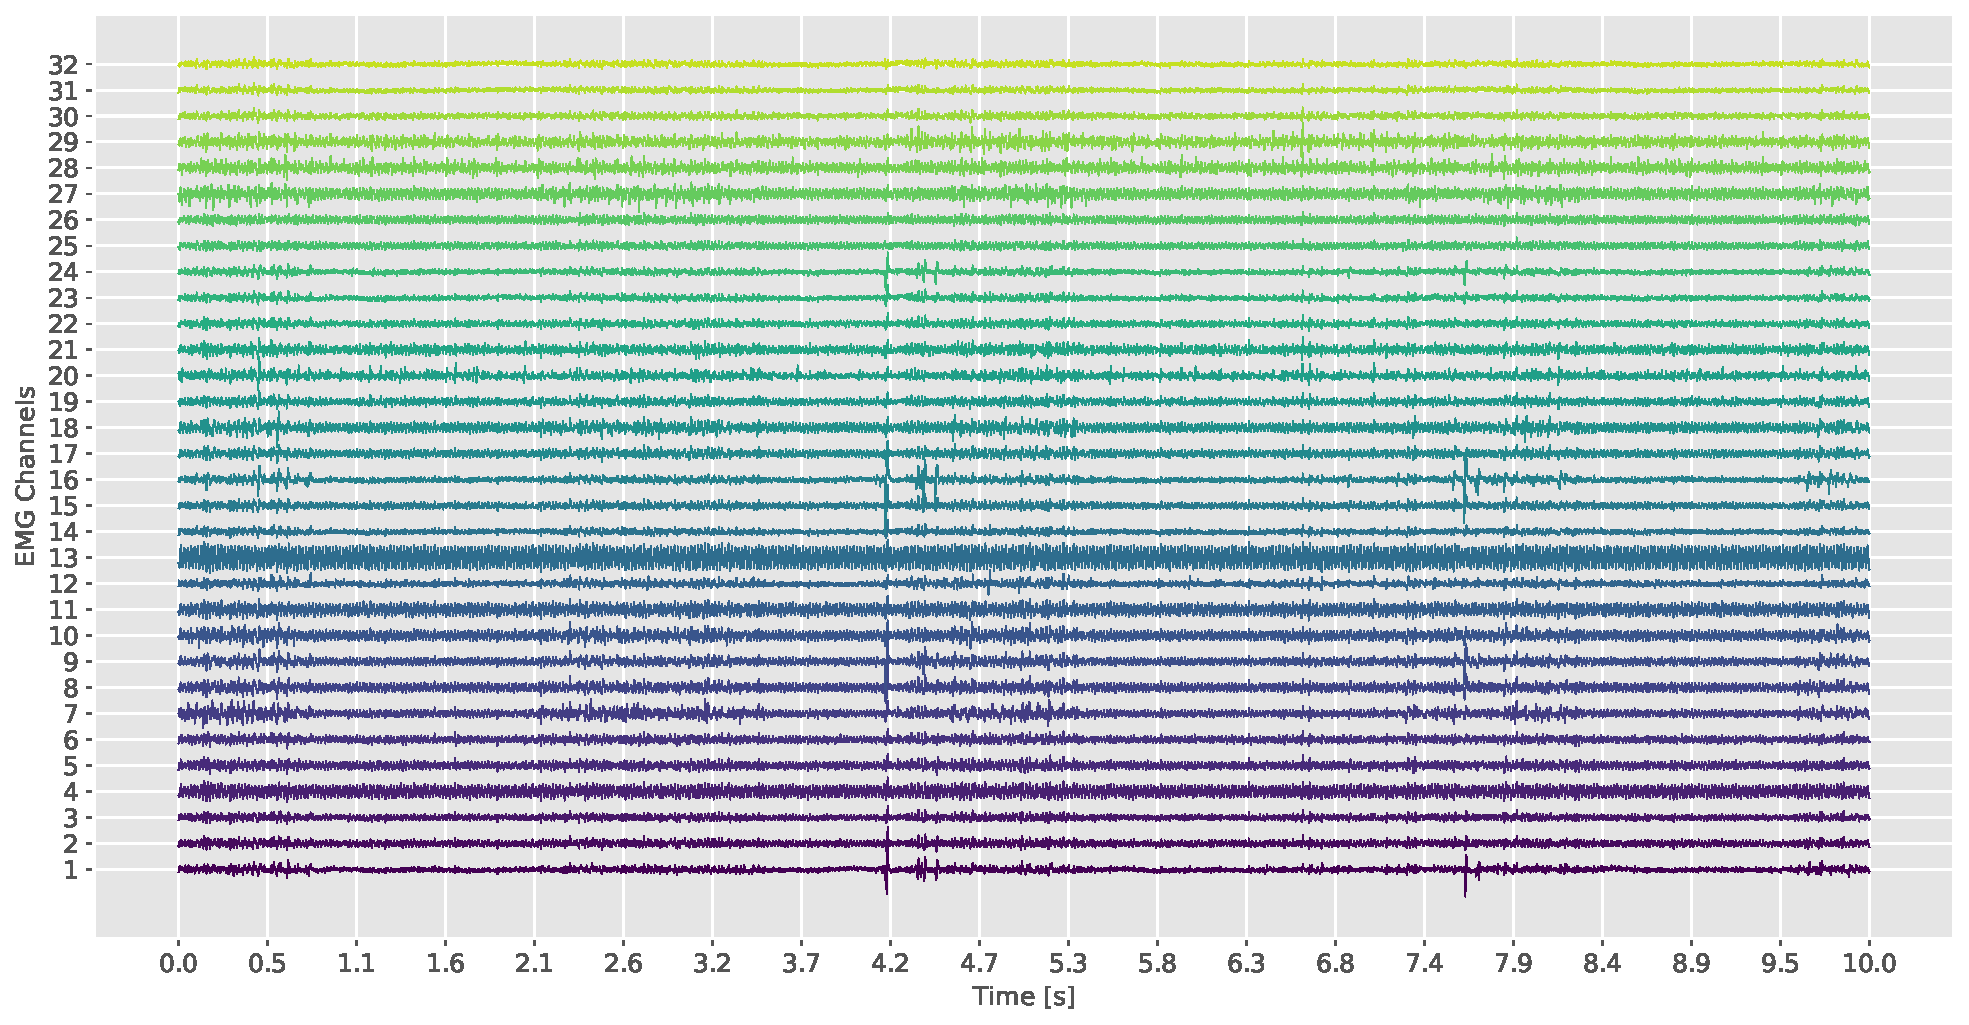
\includegraphics{images/data_analysis/fingers/raw_data.pdf}
\caption{Raw EMG data from a minimal finger flexion before
preprocessing.}
\end{figure}

\end{fignos:no-prefix-figure-caption}

\begin{fignos:no-prefix-figure-caption}

\begin{figure}
\centering
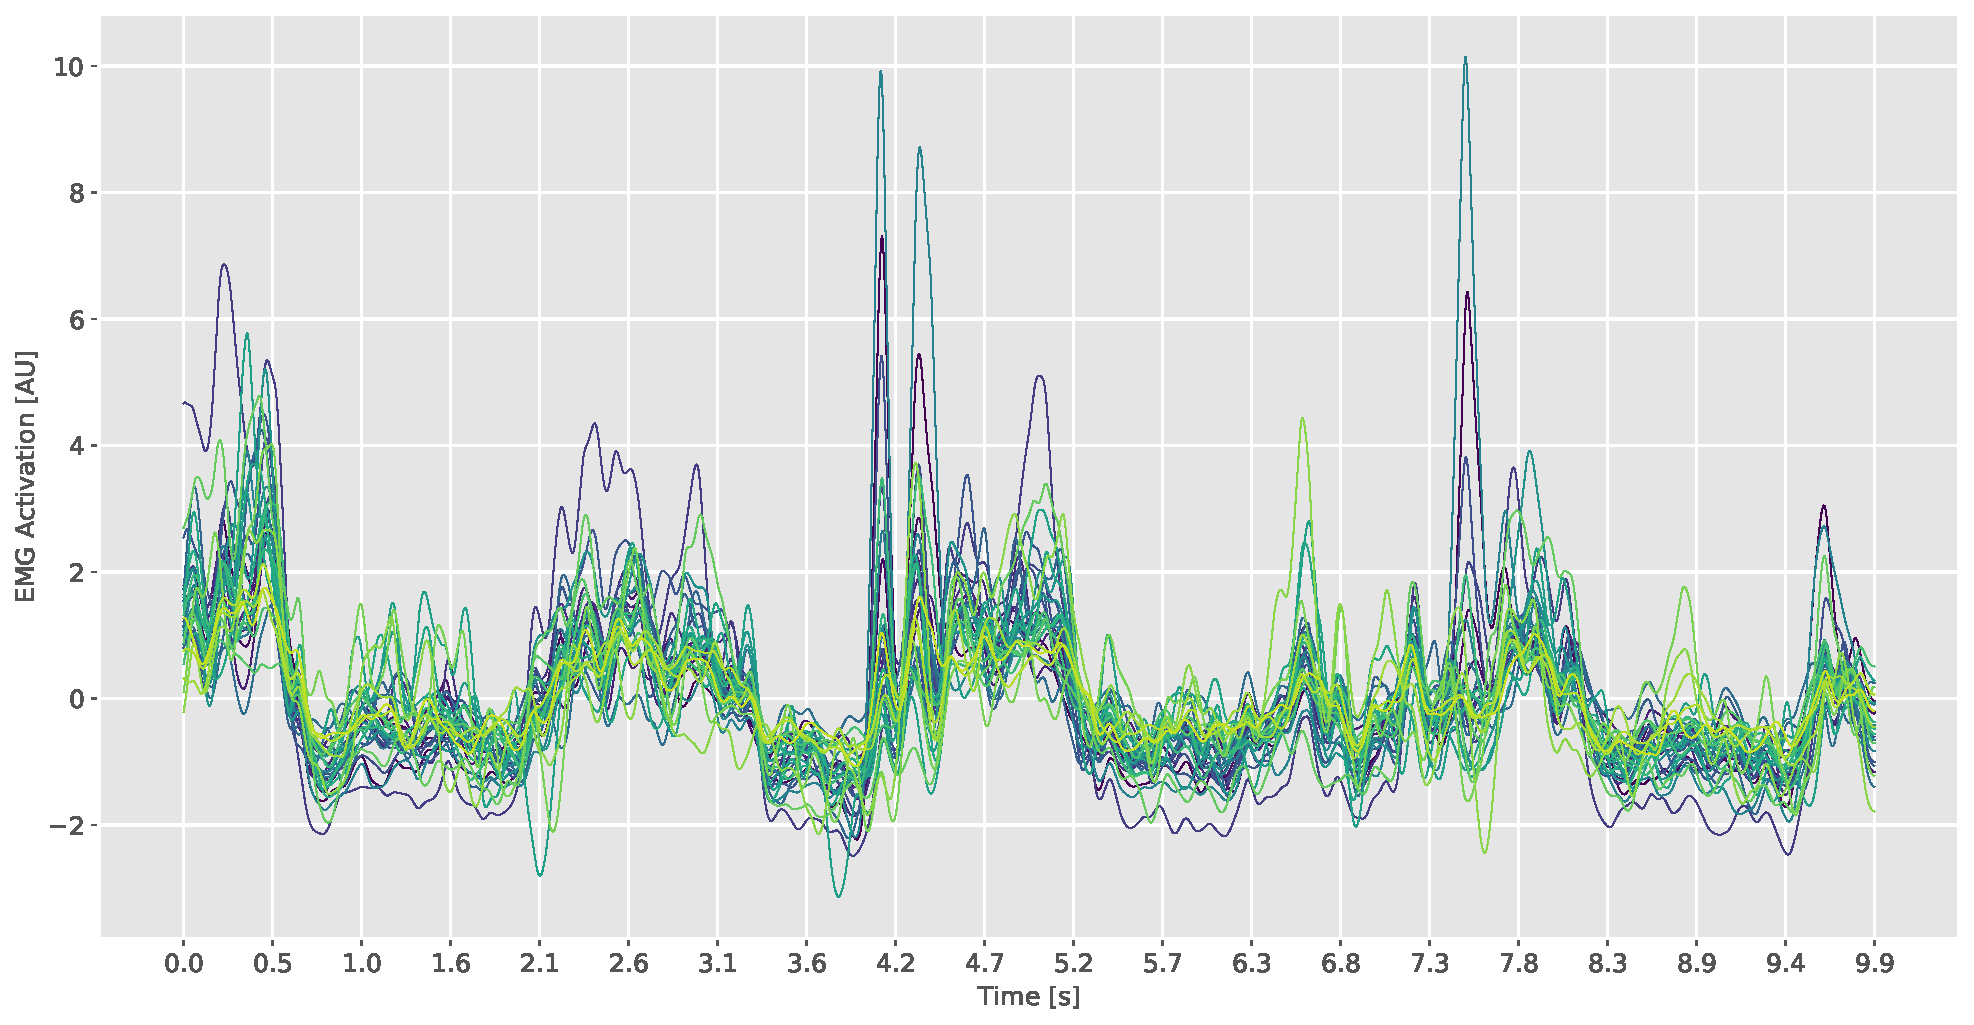
\includegraphics{images/data_analysis/fingers/preprocessed_data.pdf}
\caption{Raw EMG data from a minimal finger flexion before
preprocessing.}
\end{figure}

\end{fignos:no-prefix-figure-caption}

\begin{fignos:no-prefix-figure-caption}

\begin{figure}
\centering
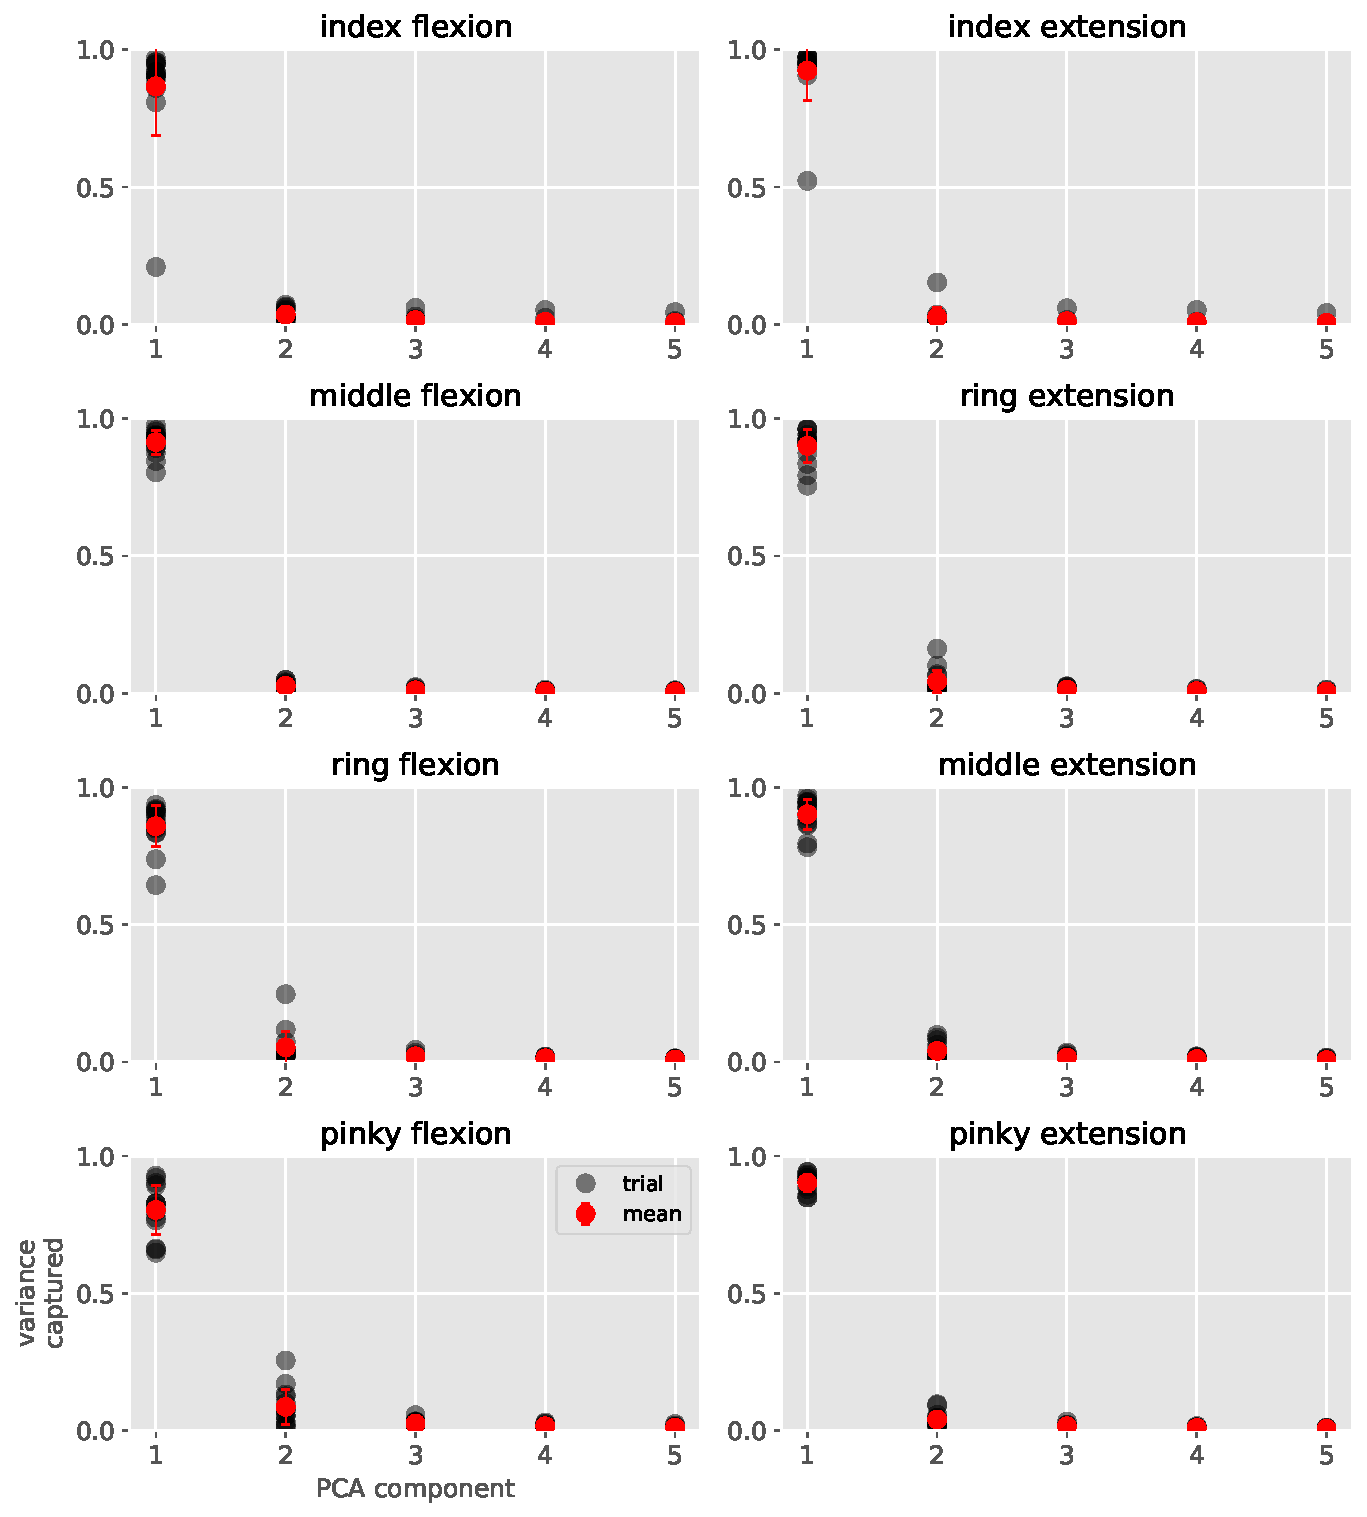
\includegraphics{images/data_analysis/fingers/PCA_variances.pdf}
\caption{Raw EMG data from a minimal finger flexion before
preprocessing.}
\end{figure}

\end{fignos:no-prefix-figure-caption}

\begin{fignos:no-prefix-figure-caption}

\begin{figure}
\centering
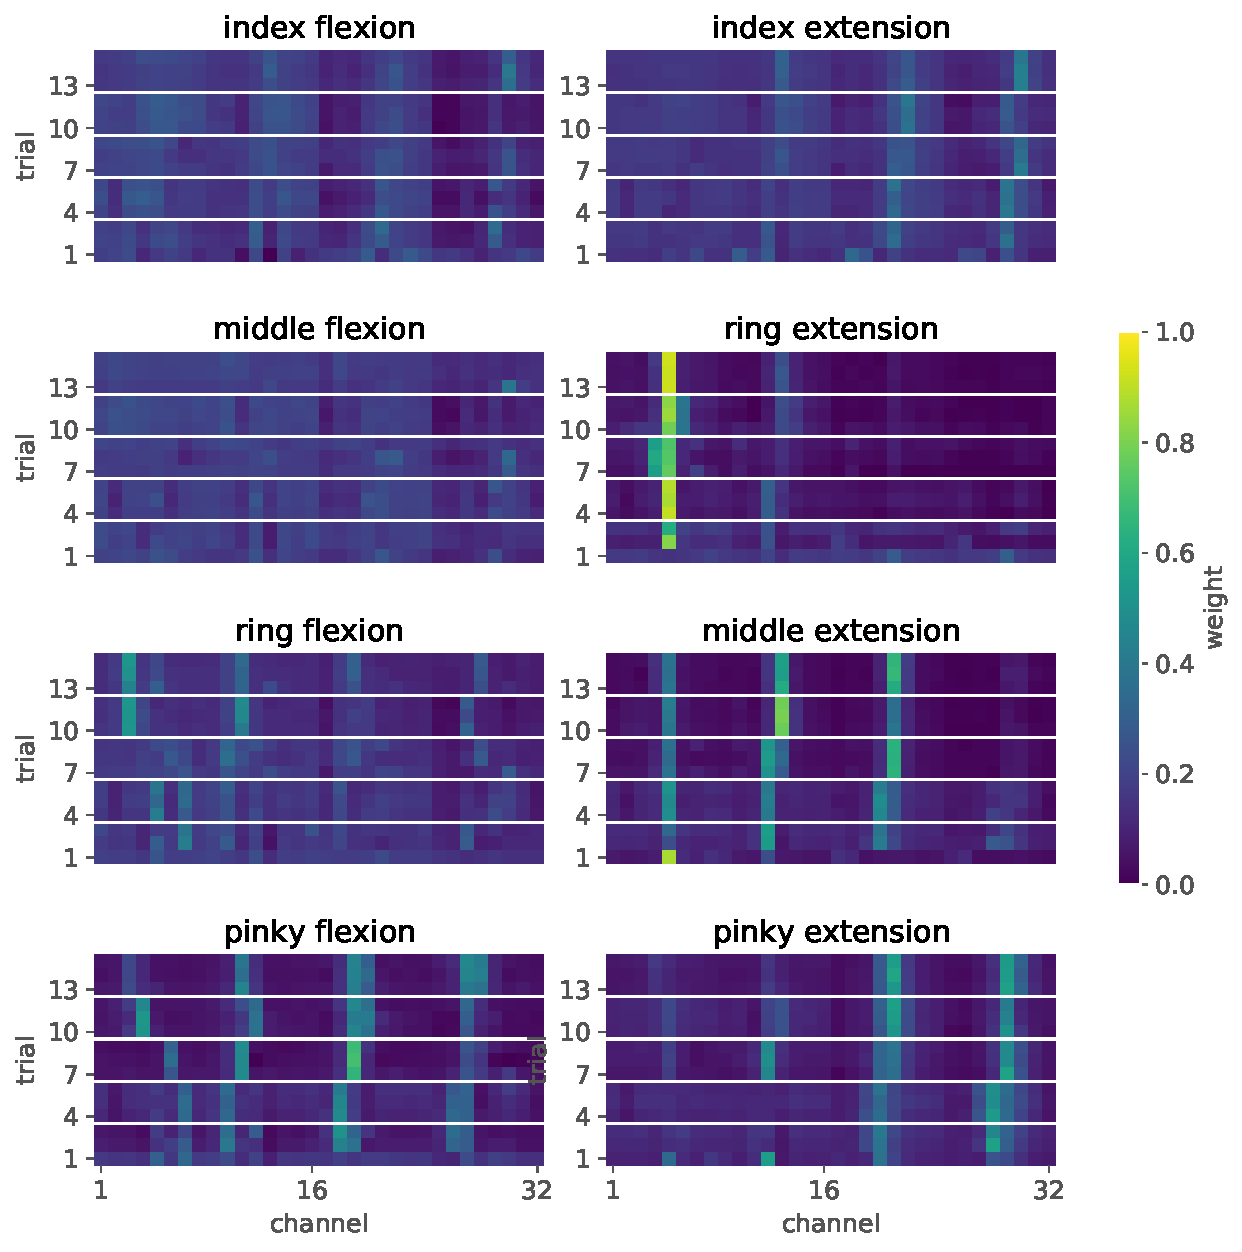
\includegraphics{images/data_analysis/fingers/PCA_components.pdf}
\caption{Raw EMG data from a minimal finger flexion before
preprocessing.}
\end{figure}

\end{fignos:no-prefix-figure-caption}

We want to determine a redundant control space from data taken during
natural activity. The difficulty with this is that such a natural
activity manifold may display spatial (channel-wise) correlations that
are possibly physiologically separable. Thus, there are two aims which
must be addressed separately:

\begin{enumerate}
\def\labelenumi{\arabic{enumi}.}
\tightlist
\item
  Expore subjects' ability to decorrelate descending output to the
  muscles which have been shown to be correlated in a natural activity
  dataset.

  \begin{itemize}
  \tightlist
  \item
    Such a structured exploration might provide support for the
    hypothesis that ``synergies'' are flexible correlations between
    muscles driven by task demands rather than (or in addition to)
    physiological structure. This needs to be done incredibly carefully
    to escape criticism of hard-wired synergy enthusiasts.
  \item
    See \emph{de Rugy 2012} for a critique of OFC and hard-wired
    synergies
  \end{itemize}
\item
  Use common correlated outputs to develop a family of BMI-type learning
  tasks as a proxy for a ``novel skill'', then track motor planning of
  this new skill to compare with motor planning algorithms.

  \begin{itemize}
  \tightlist
  \item
    We might be able to get \#1 for free by going after this goal if
    we're careful in the setup
  \item
    This is arguably a more impactful focus as it connects low-level
    motor hierarchy data (EMG) to high-level planning with a normative
    hypothesis.
  \end{itemize}
\end{enumerate}

Electrode data from a single trial of a single session is held in a data
matrix \(X\) (n\_electrodes, n\_samples), and we wish to find a latent
weight matrix \(W\) (n\_electrodes, n\_components) which reconstructs
\(X\) by projecting latent trajectories \(H\) (n\_components,
n\_samples) into electrode space:

\[
X = W\cdot{H}
\]

\(H\) is the activity of the latent processes, and \(W\) is there mixing
matrix. The columns of \(W\) are the principal vectors spanning the
latent subspace in electrode space. If we have new samples, we can
project these new points onto this subspace:

\[
h_{new} = W^T\cdot{w_{new}}
\]

To justify this decomposition, we have to make some assumptions about
the nature of the EMG signal, namely that the signal is linear
instantaneous (each EMG sample can be instantly mapped to control
space). The other assumption is that the basis \(W\) should be
orthonormal, that the columns of \(W\) are orthogonal with unity norm.
This ensures that the left inverse \(W^{-1}\) is equal to the transpose
\(W^T\) such that:

\begin{align*}
X &= W\cdot{H} \\
W^{-1}\cdot{X} &= {H} \\
W^{T}\cdot{X} &= {H}
\end{align*}

See \emph{Muceli 2014} for use of the Moore-Penrose pseudoinverse in
place of the transpose when the columns of \(W\) do not form an
orthonormal basis. This would be the case for NMF. Is there a
factorization that produces nonnegative, orthogonal coordinates? Or is
the pseudoinverse okay? I will need to test this.

Stated in an information theoretic way, we want to minimize the
reconstruction loss \(\mathcal{L}\) for our derived encoder-decoder pair
(\(E\),\(D\)). We're decoding high dimensional activity into its latent
dimensions, and encoding back into the high dimensional space. :

\[
\min_{E,D}{\mathcal{L}\left[X - EDX\right]}
\]

This way, forget about orthonormality and solve for an encoder and
decoder directly. That is, \(E\neq{D}\) is perfectly acceptable.

Each row of \(D\) might be called a \textbf{spatial filter}, a linear
combination of electrode activities into a surrogate, hopefully more
intuitive space.

In general to find such a basis we must :

\begin{itemize}
\tightlist
\item
  Extract ``natural activity manifold'' from freeform data
\item
  Use features of this natural subspace to derive control mapping

  \begin{itemize}
  \tightlist
  \item
    Linear iid features:

    \begin{itemize}
    \tightlist
    \item
      PCA
    \item
      dPCA
    \item
      NMF
    \item
      ICA
    \end{itemize}
  \item
    Linear time-dependent features:

    \begin{itemize}
    \tightlist
    \item
      SSA
    \item
      LDS model / PGM
    \end{itemize}
  \item
    Nonlinear

    \begin{itemize}
    \tightlist
    \item
      autoencoders
    \item
      networks
    \end{itemize}
  \end{itemize}
\end{itemize}

The behaviors present in our calibration dataset are crucial, as they
determine the spatial correlations used to generate the mapping. If only
complex, multi-muscle movements are present in the calibration, it will
be impossible to decode subtle movements involving few muscles.
Additionally, because extraction is unsupervised, it will be impossible
to know how to alter the control basis directions (if we wish to do so)
such that they involve single muscles or the smallest sets of muscles.

Ultimately, we want to find reproducible features in our data that are
due to muscle coordination alone, rather than volitional movements. We
want the lowest level covariance that reflects physiology rather than a
task-level behavioral description (see \emph{Todorov, Ghahramani 2005}
and \emph{Ingram, Wolpert 2009}). The idea is that if we collect data
from enough tasks, we can extract the common modes of muscle activity.
This is true only if we are sampling uniformly from the space of tasks.
Otherwise one task, and therefore one coordination pattern, will be
overrepresented.

\hypertarget{center-hold-reach-out-task}{%
\subsection{Center Hold, Reach Out
Task}\label{center-hold-reach-out-task}}

In this task, the muscles of a subject's arm are recorded using 32
channels of surface EMG. This EMG vector is mapped to a 2D force acting
on a point mass shown on the screen. The mapping
\(M\in\mathbb{R}^{2x32}\) maps 8 ``columns'' each consisting of 4
electrodes placed in a line down the length of the forearm each to one
of 2D root of unity. Each column of electrodes is thus mapped to one of
8 two-dimensional forces. Additionally, the point mass has zero inertia
and zero friction and as such displays a direct, though redundant,
readout of the EMG signal. The task asks the subject to reach one of 32
equally spaced targets on each trial.

While there are 8 possible force vectors the subject can modulate by
controlled the electrode activity on each of her 8 columns, the EMG
mapping is ultimately a projection onto the 2D plane. Since the EMG
signal is nonnegative, the subject could technically modulate just four
modes of electrode activity, the minimum number needed to span the task
space, to reach all 32 targets.

We can model the subject as selecting an EMG signal \(x\) which
minimizes the distance between a target position \(b\) and the
projection of the EMG signal through the mapping \(M\) as well as
minimizes the norm of \(x\) in order to conserve metabolic energy. This
optimization can be written as a regularized least squares problem:

\[
\min_x\frac{1}{2}||Mx - b||^2_2 + \frac{\lambda}{2}||x||_2^2.
\]

This problem is known to have a unique minimum for \(\lambda>0\) which
is an approximation \(Mx\approx b\) regardless of the shape or rank of
\(M\). This implies that the subject, if they are biophysically capable
to do so, will learn distinct motor outputs for each target rather than
reusing modes for multiple targets with different activation levels.
That is the subject will, over time, learn to fractionate their muscle
output to reach their goal in order to minimize effort. For instance, to
reach the the target at position \((1,0)\) in Cartesian coordinates, the
subject could activate a bespoke activity mode or activity the
combination of two modes for targets at \(\pm45^\circ\) from this
central target. If this is the case, the model predicts that the
dimensionality of the EMG signal will increase over the course of
training as the subject learns to construct bespoke activity modes for
each of the eight targets.

\begin{fignos:no-prefix-figure-caption}

\begin{figure}
\centering
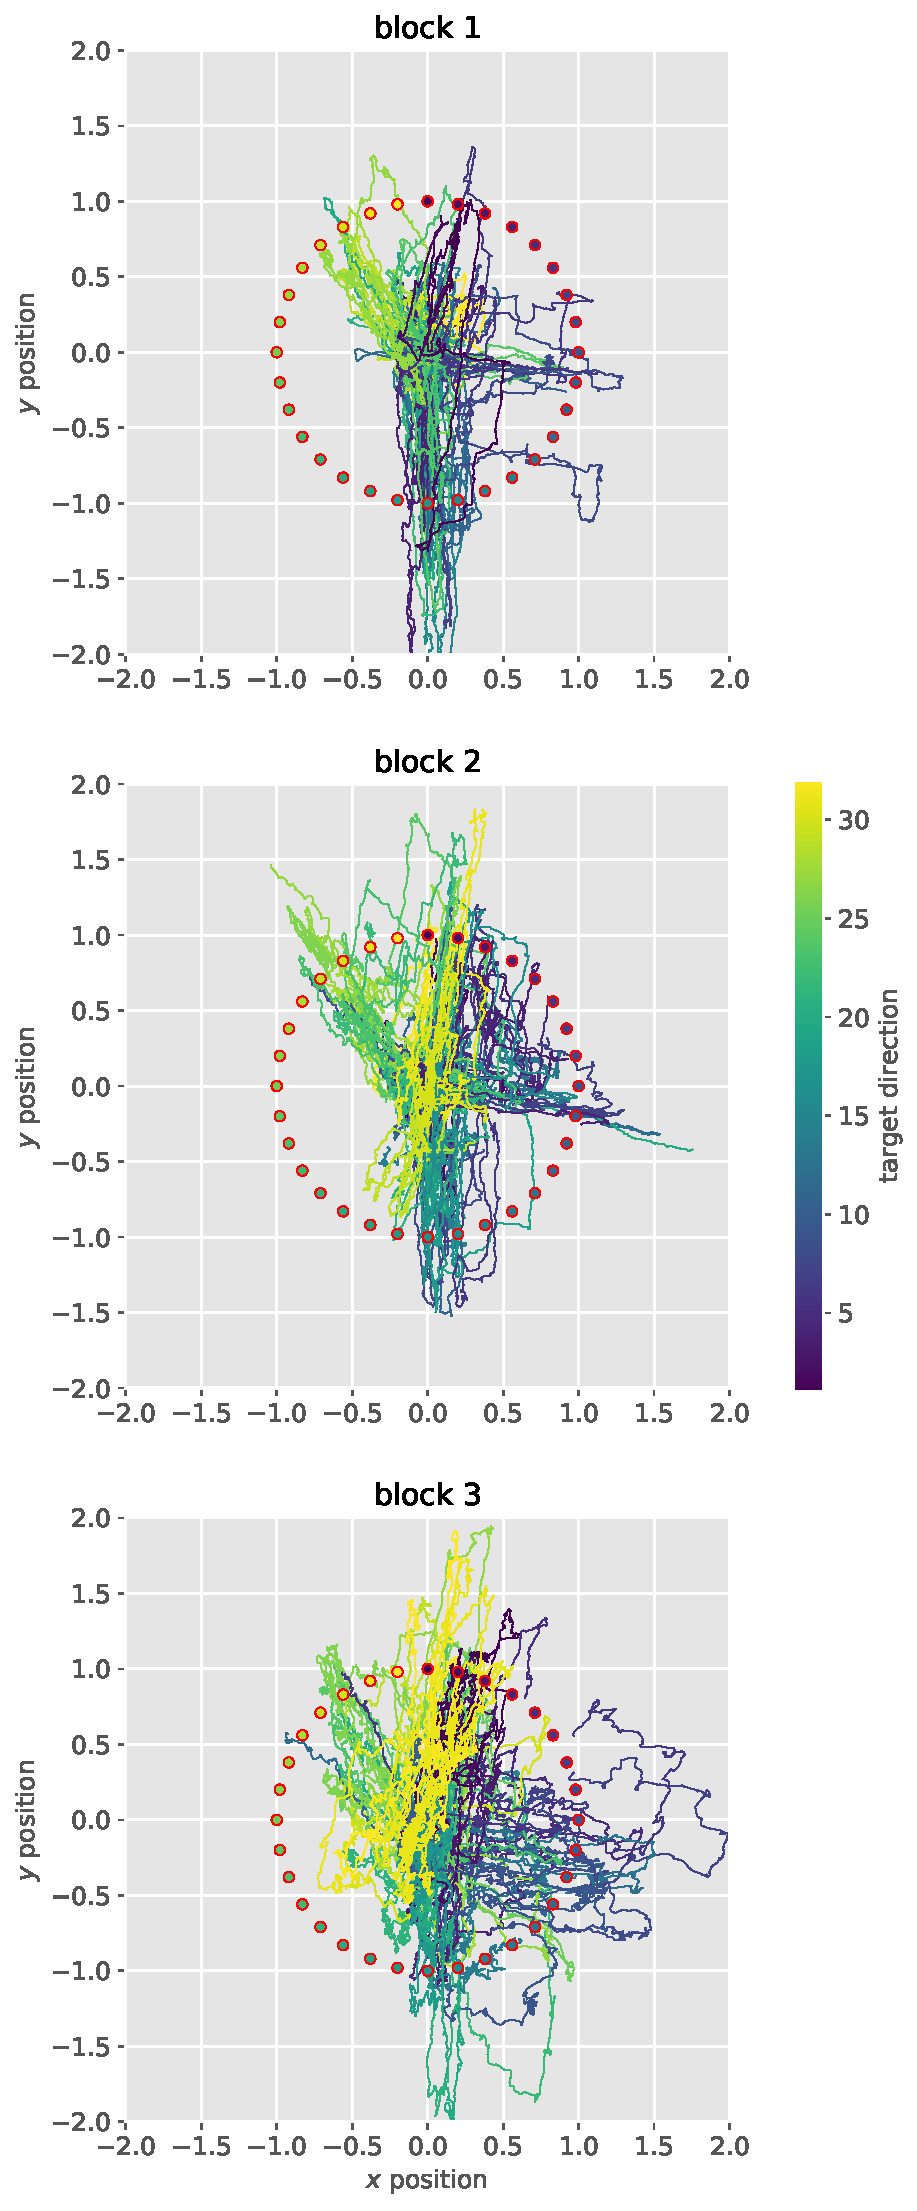
\includegraphics{images/data_analysis/center_hold/trajectories.pdf}
\caption{Point mass position trajectories in two-dimensional task space
during the center-hold, reach-out task with 8 targets spaced evenly
around the unit circle. Training was conducted over 3 blocks each with
32 trials, 4 trials per target. The first block shows roughly four
modes, the second block shows four modes more clearly, and the third
blocks may show the beginnings of fractionation.}
\end{figure}

\end{fignos:no-prefix-figure-caption}

\begin{fignos:no-prefix-figure-caption}

\begin{figure}
\centering
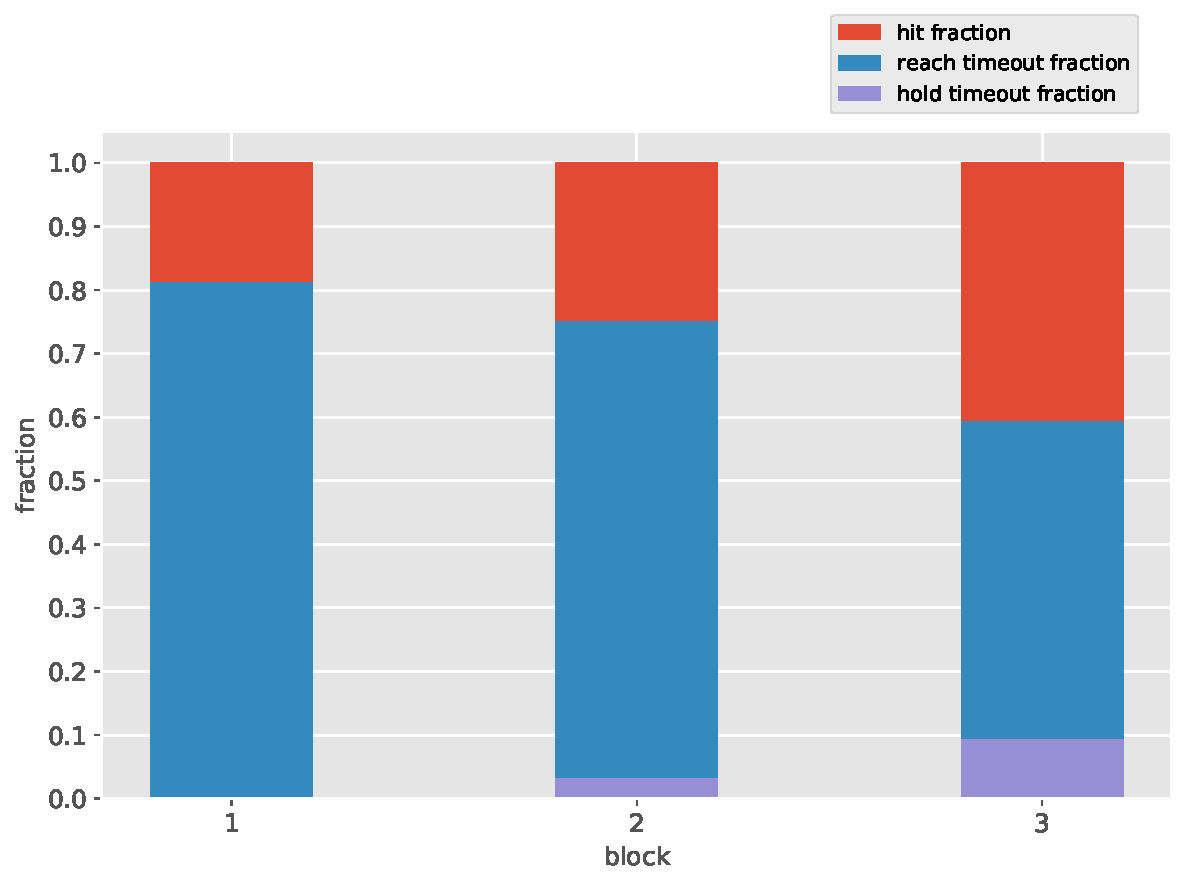
\includegraphics{images/data_analysis/center_hold/hit_fraction.pdf}
\caption{Raw EMG data from a minimal finger flexion before
preprocessing.}
\end{figure}

\end{fignos:no-prefix-figure-caption}

\begin{fignos:no-prefix-figure-caption}

\begin{figure}
\centering
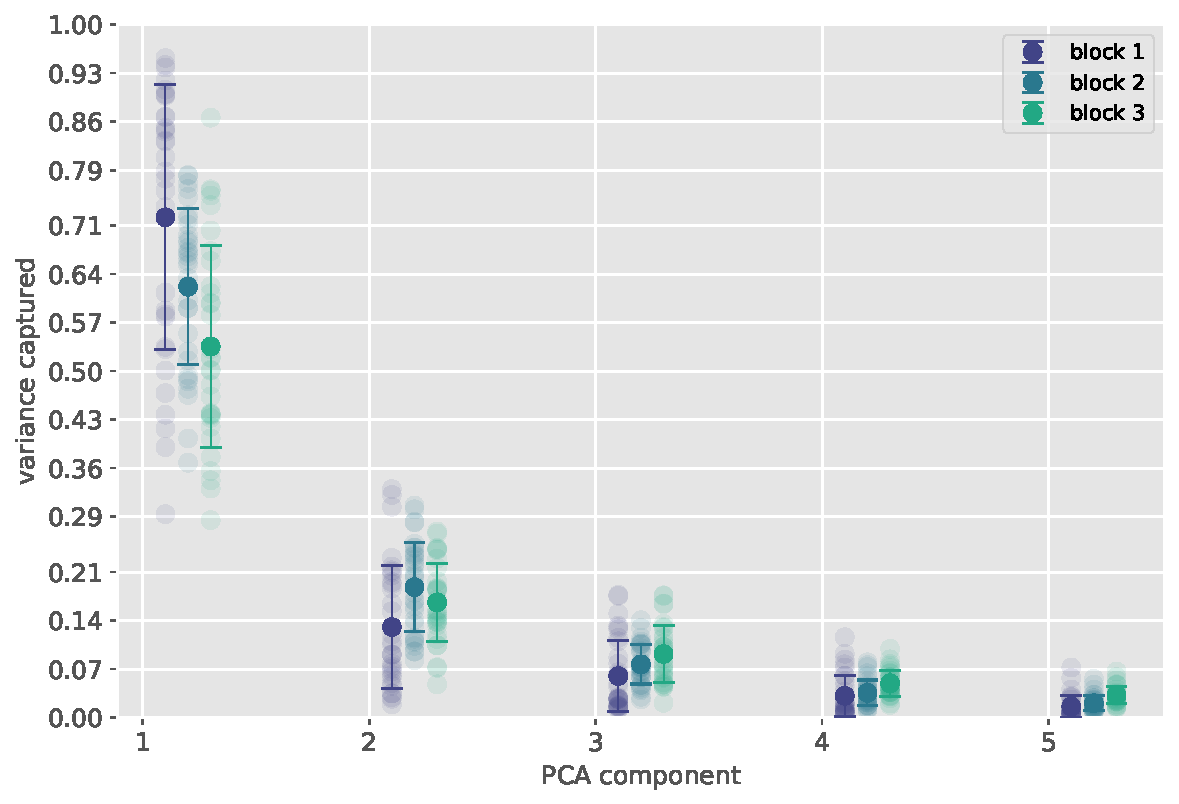
\includegraphics{images/data_analysis/center_hold/PCA_trial_variance.pdf}
\caption{Raw EMG data from a minimal finger flexion before
preprocessing.}
\end{figure}

\end{fignos:no-prefix-figure-caption}

\begin{fignos:no-prefix-figure-caption}

\begin{figure}
\centering
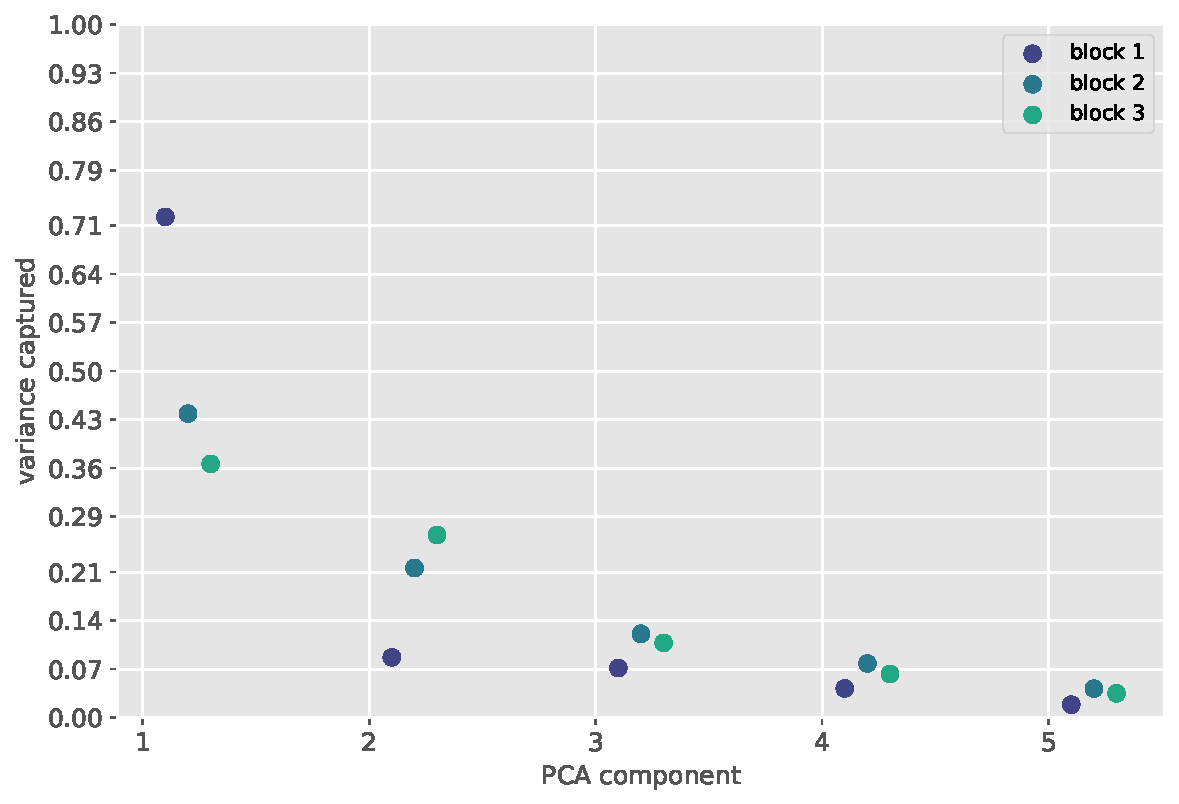
\includegraphics{images/data_analysis/center_hold/PCA_concat_variance.pdf}
\caption{Raw EMG data from a minimal finger flexion before
preprocessing.}
\end{figure}

\end{fignos:no-prefix-figure-caption}

Preliminary data for this task, through the mapping:

\[
\tilde{M} = \begin{bmatrix}M & M & M & M\end{bmatrix} \\
M =
\begin{bmatrix}
0  & 0.71  & 1   & 0.71   & 0  & -0.71  & -1  & -0.71 \\
1  & 0.71  & 0  & -0.71  & 1   & -0.71   & 0   & 0.71
\end{bmatrix}
\]

In this task, the subject's first goal is to interact through an unknown
visuomotor mapping and internalize this model. The second problem is to
use this model to solve a control problem.

\begin{enumerate}
\def\labelenumi{\arabic{enumi}.}
\tightlist
\item
  System Identification -- learning a transition function
  \(p(y_t|x_t, u_t)\)

  \begin{itemize}
  \tightlist
  \item
    How do you learn the unknown observation model from data?
  \end{itemize}
\item
  Policy Optimization

  \begin{itemize}
  \tightlist
  \item
    Once dynamics are learned (or at least stable?), how do we form a
    policy that is generalizable to new tasks under these dynamics?
  \item
    This is the control problem.
  \end{itemize}
\end{enumerate}

It's safe to assume that these processes are happening in parallel.
Because we have complete and arbitrary control over the observation
mapping, we can ask the subject to interact through a dynamic that is
intuitive (informative prior) or unintuitive (uninformative or
inhibitive prior). Each scenario, we hypothesize, will elicit different
strategies for learning and control.

The unknown mapping \(M\) from muscle to task space looks like the
observation matrix \(H\) in the LQG problem:

\begin{align*}
y_t &= Hx_t + v_t\,\,\,(\mathrm{LQG}) \\
y_t &= Mx_t + v_t. \,\,\,(\mathrm{experiment})
\end{align*}

The state dynamics in the task are of the form:

\begin{align*}
x_{t} &= Ax_{t-1} + Bu_{t-1} + w_{t-1} \,\,\,(\mathrm{LQG}) \\
x_t &= Dx_{t-1} + Iu_{t-1} + w_{t-1} \,\,\,(\mathrm{experiment})
\end{align*}

where \(D\) is a diagonal decay matrix of with terms
\(\mathrm{e}^{-\lambda}\) and \(I\) is the identity. The subject
produces muscle contractions which add to the current latent
(unobserved) state. In the absence of control signals, the state decays
back to \(0\) in line with the physics of your arm returning to a
passive state in the absence of muscle contractions. The terms \(w\) and
\(v\) are gaussian noise vectors with distributions \(\mathcal{N}(0,Q)\)
and \(\mathcal{N}(0,R)\). If we combine the transition and observation
models:

\begin{align*}
y_t &= MDx_{t-1} + Mu_{t-1} + Mw_{t-1} + v_t \\
&= A^\prime x_{t-1} + B^\prime u_{t-1} + Mw_{t-1} + v_t.
\end{align*}

We can think of this as the combined system identification problem where
\(A^\prime=MD\) and \(B^\prime=M\) are unknown and must be estimated.
The noise covariances of this altered system are now non-trivial,
however. We could also assume that the transition dynamic \(D\) is known
and that the identification problem is learning the mapping \(M\) only.
This might not be a poor assumption since the exponential decay is meant
to serve as an intuitive passive dynamic.

In each trial of the task, a subject will have some internal
representation of the observation dynamic \(M\) which may or may not be
accurate. In order to make accurate predictions, \(M\) must be
estimated.

Learning linear dynamical systems from data is a hot topic of research,
most of which seems to focus on learning in the context of complete
state observation (\(M=I\), \(y=x\)). Algorithms to determine parameters
of \(A\) and \(B\) are proposed (see Dean, Recht 2018).

From LQG theory we know that the control law is a linear function of the
state:

\begin{align*}
u_t = -L_tx_t
\end{align*}

and thus our combined system dynamic is:

\begin{align*}
y_t &= M(D-L_t)x_{t-1} + Mw_{t-1} + v_t.
\end{align*}

The noise covariance due to the observation Q is unchanged, but the new
noise covariance for the latent process is now \(MRM^T\). This may make
things difficult.

\hypertarget{sec:bg_experiment}{%
\section{Theoretical Contributions}\label{sec:bg_experiment}}

\begin{itemize}
\tightlist
\item
  how do we adapt LQR controllers trial-to-trial?
\item
  how do we use existing controllers to construct movements?
\item
  how do we construct controllers under dynamical and goal uncertainty?
\end{itemize}

\hypertarget{internal-model-adaptation-for-linear-quadratic-control}{%
\subsection{Internal Model Adaptation for Linear Quadratic
Control}\label{internal-model-adaptation-for-linear-quadratic-control}}

Here I investigate the effects of approximating internal dynamical
models for movement and using the resulting endpoint error to update
this approximation over trials.

Our state space is denoted \(x\) and our control space \(u\) where
\(dim(x) < dim(u)\). Each trial, we move from state \(x(0)\) to x(N) in
\(N\) timesteps. Each trial, we have a goal state \(x^*\) and a
resulting endpoint error \(e(N) = |x(N) - x^*|^2\).

We use a deterministic linear dynamical system to model our within-trial
state dynamics:

\[
x(t) = Ax(t-1) + Bu(t-1).
\]

For this system, we assume there exists a linear feedback control law
optimal under a given quadratic state and control cost:

\[
u(t) = Kx(t).
\]

We can write the controlled, closed-loop system dynamics for the final
time step \(N\):

\[
\begin{aligned} 
x(N) &= (A - BK)x(N-1) = Cx(N-1) \\
x(N) &= Cx(N-1) = C(Cx(N-2)) \\
x(N) &= C^Nx(0).
\end{aligned} 
\]

where \(C^N\) might be called the trajectory dynamic. If the trajectory
dynamic \(C^N\) is an approximation to the true trajectory dynamic
\(C^{N*}\), we can use the error of a given trajectory to find an
incremental update. The error at the final time step \(N\) for trial
\(r\) is

\[
e(r) = |C^N(r)x(0) - x^*|^2.
\]

This error may be due to several sources. Our internal dynamics model
\(A\) might have error relative to the true dynamic \(A^*\). Our control
gain \(K\) may be optimal relative to our internal model \(A\) but not
with respect to the true dynamic \(A^*\). Finally, we might have an
approximate model \(A\) and a suboptimal control gain \(K\). Note that
since this is still deterministic system, we have yet to include any
source of variability in state or control.

If we assume that our computation of the control gain \(K\) is optimal
for our approximate internal model \(A\) (we can compute a controller
given only our internal representation of the system dynamic being
controlled), we can use our endpoint error to derive a gradient descent
update for \(A\) on trial \(r\):

\[
A(r+1) = A(r) - \eta\frac{\partial{e(r)}}{\partial{A}}
\]

We might think about this as an internal simulation of trial \(r\)'s
trajectory, and a subsequent post hoc evaluation of the movement. To
compute \(\delta\), we must take the gradient with respect to A of the
error:

\[
\begin{aligned}
\frac{\partial{e(r)}}{\partial{A}} &= \frac{\partial{}}{\partial{A}}{|C^N(r)x(0) - x^*|^2}
\end{aligned}
\]

Since the gradient with respect to A is the same as the gradient with
respect to \(C\), we can compute the gradient with respect to C to find:

\[
% 2∑𝑁𝑘=1(𝑀𝑁𝑣−𝑤)𝑇𝑀𝑘−1𝑀𝑁−𝑘𝑣
\frac{\partial{e}}{\partial{A_{ij}}} = 2\sum_{k=1}^N\left[(C^Nx(0) - x^*)^TC^{k-1}\right]_i\left[C^{N-k}x(0)\right]_j
\]

Below is a figure showing LQR simulations across gradient descent
updates to the A matrix after it is corrupted by Gaussian noise. Each
trajectory is a single run of the LQR controlled for 200 time steps. The
star shows the target state, the colored circles show the endpoints of
the trajectories. The red circle is the initial state.

\begin{figure}
\hypertarget{fig:gradient_descent}{%
\centering
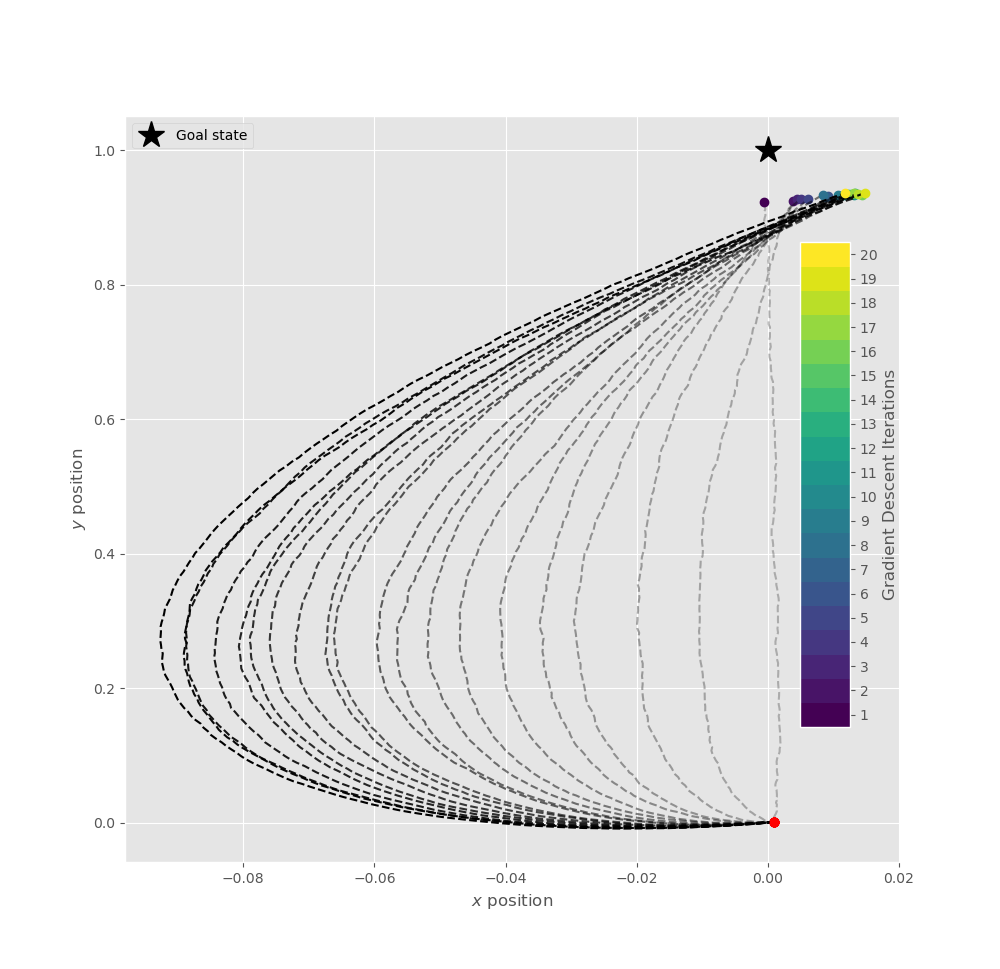
\includegraphics{images/simulations/gradient_descent_on_A.png}
\caption{Iterations of gradient descent on the \(A\) matrix of an
infinite-horizon LQR. Each dotted line in a trajectory with a different
\(A\) matrix. The red circle denotes the initial state, the star denotes
the goal state, and the colored circles denote the endpoints of each
iteration.}\label{fig:gradient_descent}
}
\end{figure}

The descent is converging in endpoint error in position, velocity, and
force space. Unfortunately, this optimization is causing the dynamics to
change. The routine is also very fragile to parameter changes. Next
steps:

\begin{itemize}
\tightlist
\item
  Gain a better understanding of the loss landscape, including it's
  degeneracy. It may be possible to compute the optimum analytically.
\item
  Corrupt the \(A\) matrix in a more principled way, working to alter
  the passive dynamics in a physically realistic manner.
\item
  Explore the action of the resulting gradient through it's eigenvalues
  and vectors. This can be done in two dimensions as a starting point.
\item
  Compute second-order derivatives and work towards a Newton's method.
\item
  Compute derivatives with respect to the control law \(K\) as a
  comparison.
\item
  Analyze results of the routine in comparison with the reaching
  adaptation literature.
\end{itemize}

Think more about subspaces - preparatory activity in one subspsce,
online control in another? - learning in one subspace but not another? -
compression of model to a subspace?

\hypertarget{policy-selection}{%
\subsection{Policy Selection}\label{policy-selection}}

each timestep you combine actions from component policies to choose an
action

Here we'll review and discuss models of action selection and policy
composition as a means of theorizing about how subjects learn novel
skills.

In a sense, we're setting up several different directions for our
understanding of composition and action selection which can be
experimentally tested.

We have a direct selection algorithm, composition through policy
addition, and composition through policy multiplication.

\hypertarget{kl-control-composition-1-day}{%
\subsubsection{KL-control Composition (1
day)}\label{kl-control-composition-1-day}}

This setup is particular subset of OFC problems.

Dynamics Cost

Composable policies

PLOT OF INTUITIVE EXAMPLE

\hypertarget{temporal-composition}{%
\subsubsection{Temporal Composition}\label{temporal-composition}}

there is a spectrum of latency in the feedback response

can different controllers be used for different latencies, and adjusted
accordingly?

\hypertarget{generalized-policy-selection-1-day}{%
\subsubsection{Generalized Policy Selection (1
day)}\label{generalized-policy-selection-1-day}}

This is in the MDP case

Learning happens in several ways-- reward regression, Q-learning

What are rewards? What are tasks? What are actions?

Is GPI with LQRs / LQR-RL a good model for motor learning? Define a
model and see if it recapitulates known motor learning phenomena on
existing experiments + accounts for things that previous models don't.
(Similar in spirit to Geerts et al.~(2020)). Can this model track the
higher-order statistics of trajectories during motor learning?

\hypertarget{model-based-reinforcement-learning}{%
\subsubsection{Model-based Reinforcement
Learning}\label{model-based-reinforcement-learning}}

Since we only have an approximate model of the system dynamic, we could
simply work towards an optimal policy directly using gradient
derivative-free optimization methods in a model-free approach. Since we
have good evidence that humans leverage internal models to make
decisions (at least in a motor problem domain), we need to define an
algorithm which uses past observations and controls to update our
approximation for the system dynamic. Here is a very general algorithm:

\begin{enumerate}
\def\labelenumi{\arabic{enumi}.}
\setcounter{enumi}{-1}
\tightlist
\item
  Define a base policy/controller and base system model (\(L_0\) and
  \(\hat{M}_0\))
\item
  Collect samples (by interacting with the true environment
  \(M_{true}\)) using the current policy/controller (collect
  \(y_t,u_t,y_{t+1}\) triples using \(L_i\) for \(i \in \{0\dots N\}\)
\item
  Use sample(s) / trajectories to update current system dynamical model
  \(\hat{M}_i\)
\item
  Update current policy/controller \(L_i\) (using the system dynamics or
  using a direct policy method)
\end{enumerate}

If the true system dynamics were known, we could solve the Algebraic
Riccati Equation with a backwards pass, and compute our controls in a
forward pass. This general algorithm structure highlights how the
(unknown) system identification and controller design are intertwined:
identifying a system appropriately must rely on sampling and fitting
regions of the state space pertinent to adequate control in terms of
cost (Ross ICML 2012). Otherwise, our approximation to the true system
dynamic will only produce a valid controller in regions we have
previously explored. The question is how we can effectively (sample and
time efficiently) utilize new state transitions we encounter either
online as feedback or between trials to update our model and policy.
That is, the number of trials and/or trajectories to use before updating
either the system model and/or policy is an important parameter.

In the LQG setting, this might be called ``adaptive LQG''.

\hypertarget{internal-model-adaptation-for-linear-quadratic-control}{%
\subsection{Internal Model Adaptation for Linear Quadratic
Control}\label{internal-model-adaptation-for-linear-quadratic-control}}

Here I investigate the effects of approximating internal dynamical
models for movement and using the resulting endpoint error to update
this approximation over trials.

Our state space is denoted \(x\) and our control space \(u\) where
\(dim(x) < dim(u)\). Each trial, we move from state \(x(0)\) to x(N) in
\(N\) timesteps. Each trial, we have a goal state \(x^*\) and a
resulting endpoint error \(e(N) = |x(N) - x^*|^2\).

We use a deterministic linear dynamical system to model our within-trial
state dynamics:

\[
x(t) = Ax(t-1) + Bu(t-1).
\]

For this system, we assume there exists a linear feedback control law
optimal under a given quadratic state and control cost:

\[
u(t) = Kx(t).
\]

We can write the controlled, closed-loop system dynamics for the final
time step \(N\):

\[
\begin{aligned} 
x(N) &= (A - BK)x(N-1) = Cx(N-1) \\
x(N) &= Cx(N-1) = C(Cx(N-2)) \\
x(N) &= C^Nx(0).
\end{aligned} 
\]

where \(C^N\) might be called the trajectory dynamic. If the trajectory
dynamic \(C^N\) is an approximation to the true trajectory dynamic
\(C^{N*}\), we can use the error of a given trajectory to find an
incremental update. The error at the final time step \(N\) for trial
\(r\) is

\[
e(r) = |C^N(r)x(0) - x^*|^2.
\]

This error may be due to several sources. Our internal dynamics model
\(A\) might have error relative to the true dynamic \(A^*\). Our control
gain \(K\) may be optimal relative to our internal model \(A\) but not
with respect to the true dynamic \(A^*\). Finally, we might have an
approximate model \(A\) and a suboptimal control gain \(K\). Note that
since this is still deterministic system, we have yet to include any
source of variability in state or control.

If we assume that our computation of the control gain \(K\) is optimal
for our approximate internal model \(A\) (we can compute a controller
given only our internal representation of the system dynamic being
controlled), we can use our endpoint error to derive a gradient descent
update for \(A\) on trial \(r\):

\[
A(r+1) = A(r) - \eta\frac{\partial{e(r)}}{\partial{A}}
\]

We might think about this as an internal simulation of trial \(r\)'s
trajectory, and a subsequent post hoc evaluation of the movement. To
compute \(\delta\), we must take the gradient with respect to A of the
error:

\[
\begin{aligned}
\frac{\partial{e(r)}}{\partial{A}} &= \frac{\partial{}}{\partial{A}}{|C^N(r)x(0) - x^*|^2}
\end{aligned}
\]

Since the gradient with respect to A is the same as the gradient with
respect to \(C\), we can compute the gradient with respect to C to find:

\[
% 2∑𝑁𝑘=1(𝑀𝑁𝑣−𝑤)𝑇𝑀𝑘−1𝑀𝑁−𝑘𝑣
\frac{\partial{e}}{\partial{A_{ij}}} = 2\sum_{k=1}^N\left[(C^Nx(0) - x^*)^TC^{k-1}\right]_i\left[C^{N-k}x(0)\right]_j
\]

Below is a figure showing LQR simulations across gradient descent
updates to the A matrix after it is corrupted by Gaussian noise. Each
trajectory is a single run of the LQR controlled for 200 time steps. The
star shows the target state, the colored circles show the endpoints of
the trajectories. The red circle is the initial state.

\begin{figure}
\hypertarget{fig:gradient_descent}{%
\centering
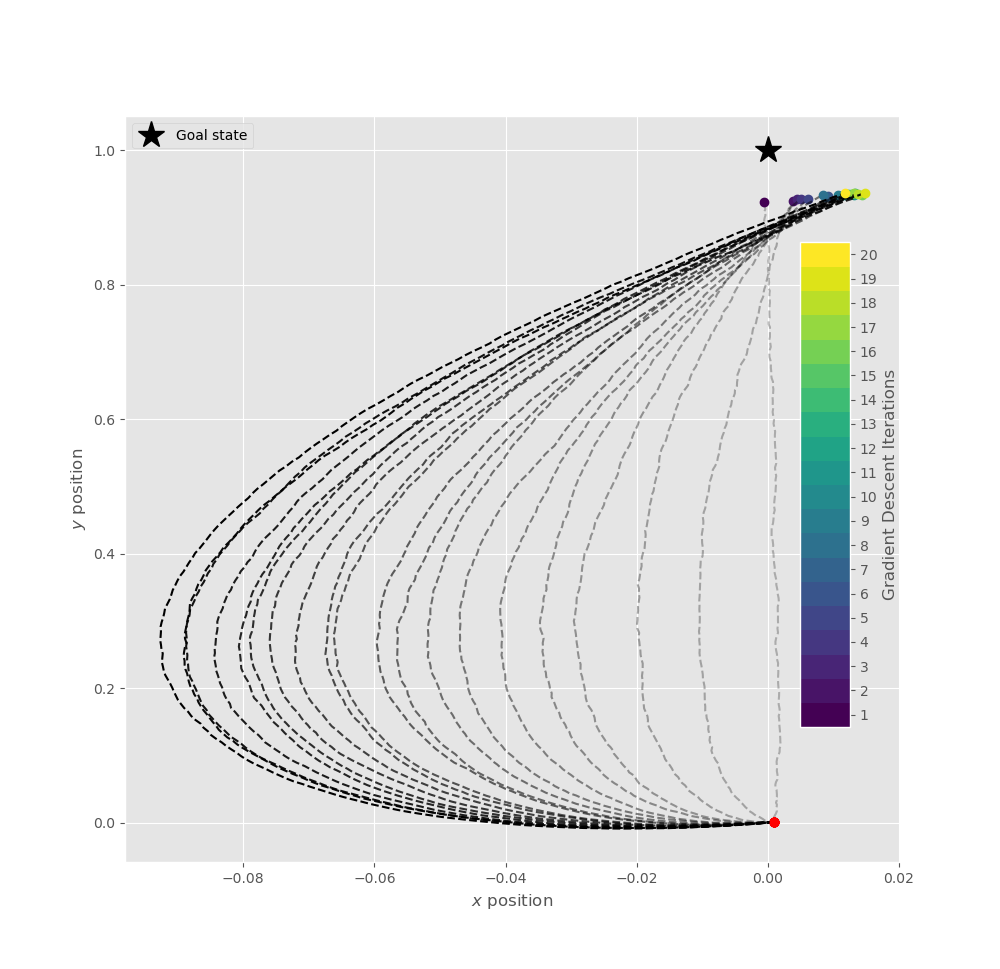
\includegraphics{images/simulations/gradient_descent_on_A.png}
\caption{Iterations of gradient descent on the \(A\) matrix of an
infinite-horizon LQR. Each dotted line in a trajectory with a different
\(A\) matrix. The red circle denotes the initial state, the star denotes
the goal state, and the colored circles denote the endpoints of each
iteration.}\label{fig:gradient_descent}
}
\end{figure}

The descent is converging in endpoint error in position, velocity, and
force space. Unfortunately, this optimization is causing the dynamics to
change. The routine is also very fragile to parameter changes. Next
steps:

\begin{itemize}
\tightlist
\item
  Gain a better understanding of the loss landscape, including it's
  degeneracy. It may be possible to compute the optimum analytically.
\item
  Corrupt the \(A\) matrix in a more principled way, working to alter
  the passive dynamics in a physically realistic manner.
\item
  Explore the action of the resulting gradient through it's eigenvalues
  and vectors. This can be done in two dimensions as a starting point.
\item
  Compute second-order derivatives and work towards a Newton's method.
\item
  Compute derivatives with respect to the control law \(K\) as a
  comparison.
\item
  Analyze results of the routine in comparison with the reaching
  adaptation literature.
\end{itemize}

\hypertarget{next-steps}{%
\section{Next Steps}\label{next-steps}}

Big Things

First completing a methodsy style piece of owrk about the setup,
illlustrating the generation of bespoke control strategies by careful
tracking of the EMG modes relative to task performance.

Next is to work on models of learning by extending the framework of OFC
through additions of composition and error-based adaptation.

\hypertarget{data-collection-at-scale}{%
\subsection{Data Collection at Scale}\label{data-collection-at-scale}}

\begin{itemize}
\tightlist
\item
  scale up data collection with more subjects across many days
\item
  intersubject differences
\end{itemize}

\hypertarget{data-analysis}{%
\subsubsection{Data Analysis}\label{data-analysis}}

Our preliminary data confirms the working principle of the setup and
highlights the next steps for producing a quality dataset.

Address the noise concerns in the data -- better hardware, should be
very low noise relative to our signal.

\begin{itemize}
\item
  more advanced EMG analyses in the task setting

  \begin{itemize}
  \tightlist
  \item
    autoencoders (farina
    paper)\textsuperscript{\protect\hyperlink{ref-vujaklijaOnlineMappingEMG2018}{71}}
  \item
    bayesian inference techniques bespoke for EMG signals -- pull out
    control modes

    \begin{itemize}
    \tightlist
    \item
      choosing different aspects of the data model for inference

      \begin{itemize}
      \tightlist
      \item
        what kind of priors for tunings, latent space,
      \item
        we would need some kind of round truth? a different
        experiment\ldots{}
      \end{itemize}
    \end{itemize}
  \end{itemize}
\item
  better techniques for developing mappings
\item
  long-range correlations in the data, correlation functions

  \begin{itemize}
  \tightlist
  \item
    \textsuperscript{\protect\hyperlink{ref-crevecoeurGoldstandardApproachAddress2010}{72}}
  \end{itemize}
\item
  Dynamical modes in the data using dynamical systems analysis
  techniques
\end{itemize}

\hypertarget{task-design}{%
\subsubsection{Task Design}\label{task-design}}

\begin{itemize}
\tightlist
\item
  formalize specific task designs which link with our theoretical
  interests
\end{itemize}

\hypertarget{optimization}{%
\subsubsection{Optimization}\label{optimization}}

we want to stay close to models, testing them as we go - optimization
models (regularized regression) -- pure force learning - perturbations
of this + predictions? mapping perturbation, noise perturbations

\hypertarget{optimal-control}{%
\subsubsection{Optimal Control}\label{optimal-control}}

\begin{itemize}
\tightlist
\item
  stochastic optimal control model comparisons

  \begin{itemize}
  \tightlist
  \item
    cost models
  \item
    perturbations in goal
  \item
    go-before you know / goal uncertainty
  \item
    noise perturbations -- do reponses match the models?
  \end{itemize}
\item
  dynamics model fitting

  \begin{itemize}
  \tightlist
  \item
    internal model uncertainty
  \item
    modeled with robust optimal control?
  \end{itemize}
\end{itemize}

stochastic control vs.~robust control vs.~adaptive control

learning control over trials learning control via reward
(RL)\textsuperscript{\protect\hyperlink{ref-vanderkooijLearningReachTrajectory2021}{73}}
constructing control from primitives for transfer (GPS, KL-control)

\hypertarget{eye-tracking}{%
\subsection{Eye Tracking}\label{eye-tracking}}

Active learning, perception + action

\hypertarget{open-questions}{%
\subsection{Open Questions}\label{open-questions}}

The following questions need answers, to make progress we must form
hypotheses around the most pressing of these questions and design
experiments to test these hypotheses.

\begin{itemize}
\item
  how does a subject sample the state space as to efficiently learn? do
  they sample optimally? how does controller/policy optimization proceed
  based on system identification?
\item
  how does a human subject use error information from each trial and
  feedback from each time step to update their model and/or policy?

  \begin{itemize}
  \tightlist
  \item
    how does a subject balance policy updates with model updates?
  \end{itemize}
\item
  On what scale (trials, timesteps) is the model altered? the policy?

  \begin{itemize}
  \tightlist
  \item
    Replanning at every timestep is a model predictive control algorithm
  \item
    What prediction can we make for ID/learning every trial?
  \end{itemize}
\item
  how does a subject avoid ``distribution mismatch'' between their base
  policy and their optimal policy? How do they efficiently explore and
  use this new data to update their internal model?

  \begin{itemize}
  \tightlist
  \item
    what exploration strategy does a subject use to avoid mismatch?
  \item
    what
  \end{itemize}
\item
  What is a subject's baseline/prior model?
  \(y_{t} = \hat{f}_0(x_t,u_t)\) or \(y_{t} \propto p_0(y_t|x_{t},u_t)\)
\item
  What is the base policy / prior policy? \(u_t = \pi_0(\hat{x}_t)\)
\item
  How do we think about learning a distribution over trajectories in
  control law space, or perhaps equivalently, in covariance/precision
  space?
\item
  We might hypothesize that a subject will act as randomly as possible
  while minimizing cost, a maximum entropy solution that converges to an
  optimal controller? \(\mathcal{H}(p(u_t|x_t))\)
\item
  How does a subject penalize changes to their controllers? Do they
  follow a KL-divergence type of measurement when improving their
  policy?
\item
  In a behavioral experiment, how can you disentangle system
  identification/estimation and control? Is suboptimality due to one or
  the other?
\item
  How does the observation mapping relate to the latent state
  covariance? The task state covariance?
\item
  How do we formalize this into a probabilistic graphical model? Why
  would we?

  \begin{itemize}
  \tightlist
  \item
    Would this make it easier to reason about what the goals are?
  \item
    Would learning \(M\) become an inference problem?
  \item
    Would solving the control problem become an inference problem\ldots?
  \end{itemize}
\item
  What noise assumptions can we make? Can we not make?

  \begin{itemize}
  \tightlist
  \item
    How can we incorporate signal-dependent noise?
  \end{itemize}
\end{itemize}

\newpage

\hypertarget{bibliography}{%
\subsection*{Bibliography}\label{bibliography}}
\addcontentsline{toc}{subsection}{Bibliography}

\hypertarget{refs}{}
\begin{CSLReferences}{0}{0}
\leavevmode\hypertarget{ref-McNamee2019}{}%
\CSLLeftMargin{1. }
\CSLRightInline{McNamee, D. \& Wolpert, D. M. Internal {Models} in
{Biological Control}. \emph{Annual Review of Control, Robotics, and
Autonomous Systems} \textbf{2}, 339--364 (2019).}

\leavevmode\hypertarget{ref-Todorov2004}{}%
\CSLLeftMargin{2. }
\CSLRightInline{Todorov, E. Optimality principles in sensorimotor
control. \emph{Nature Neuroscience} \textbf{7}, 907--915 (2004).}

\leavevmode\hypertarget{ref-koberReinforcementLearningRobotics2013}{}%
\CSLLeftMargin{3. }
\CSLRightInline{Kober, J., Bagnell, J. A. \& Peters, J. Reinforcement
learning in robotics: {A} survey. \emph{The International Journal of
Robotics Research} \textbf{32}, 1238--1274 (2013).}

\leavevmode\hypertarget{ref-sauerbreiCorticalPatternGeneration2019}{}%
\CSLLeftMargin{4. }
\CSLRightInline{Sauerbrei, B. A. \emph{et al.} Cortical pattern
generation during dexterous movement is input-driven. \emph{Nature}
(2019)
doi:\href{https://doi.org/10.1038/s41586-019-1869-9}{10.1038/s41586-019-1869-9}.}

\leavevmode\hypertarget{ref-Bernstein1967}{}%
\CSLLeftMargin{5. }
\CSLRightInline{Bernstein, N. \emph{The coordination and regulation of
movements}. ({Pergamon}, 1967).}

\leavevmode\hypertarget{ref-kitanoBiologicalRobustness2004}{}%
\CSLLeftMargin{6. }
\CSLRightInline{Kitano, H. Biological robustness. \emph{Nature Reviews
Genetics} \textbf{5}, 826--837 (2004).}

\leavevmode\hypertarget{ref-fuglevandMechanicalPropertiesNeural2011}{}%
\CSLLeftMargin{7. }
\CSLRightInline{Fuglevand, A. J. Mechanical properties and neural
control of human hand motor units: {Control} of human hand motor units.
\emph{The Journal of Physiology} \textbf{589}, 5595--5602 (2011).}

\leavevmode\hypertarget{ref-harrisSignaldependentNoiseDetermines1998}{}%
\CSLLeftMargin{8. }
\CSLRightInline{Harris, C. M. \& Wolpert, D. M. Signal-dependent noise
determines motor planning. \emph{Nature} \textbf{394}, 780--784 (1998).}

\leavevmode\hypertarget{ref-vanduinenConstraintsControlHuman2011}{}%
\CSLLeftMargin{9. }
\CSLRightInline{van Duinen, H. \& Gandevia, S. C. Constraints for
control of the human hand: {Control} of the hand. \emph{The Journal of
Physiology} \textbf{589}, 5583--5593 (2011).}

\leavevmode\hypertarget{ref-Valero-Cuevas2007}{}%
\CSLLeftMargin{10. }
\CSLRightInline{Valero-Cuevas, F. J. \emph{et al.} The tendon network of
the fingers performs anatomical computation at a macroscopic scale.
\emph{IEEE Transactions on Biomedical Engineering} \textbf{54},
1161--1166 (2007).}

\leavevmode\hypertarget{ref-yanUnexpectedComplexityEveryday2020}{}%
\CSLLeftMargin{11. }
\CSLRightInline{Yan, Y., Goodman, J. M., Moore, D. D., Solla, S. A. \&
Bensmaia, S. J. Unexpected complexity of everyday manual behaviors.
\emph{Nature Communications} \textbf{11}, 3564 (2020).}

\leavevmode\hypertarget{ref-Basmajian1963}{}%
\CSLLeftMargin{12. }
\CSLRightInline{Basmajian, J. V. Control and {Training} of {Individual
Motor Units}. \emph{Science} \textbf{141}, 440--441 (1963).}

\leavevmode\hypertarget{ref-merelHierarchicalMotorControl2019}{}%
\CSLLeftMargin{13. }
\CSLRightInline{Merel, J., Botvinick, M. \& Wayne, G. Hierarchical motor
control in mammals and machines. \emph{Nature Communications}
\textbf{10}, 5489 (2019).}

\leavevmode\hypertarget{ref-DAvella2003}{}%
\CSLLeftMargin{14. }
\CSLRightInline{D'Avella, A., Saltiel, P. \& Bizzi, E. Combinations of
muscle synergies in the construction of a natural motor behavior.
\emph{Nature Neuroscience} \textbf{6}, 300--308 (2003).}

\leavevmode\hypertarget{ref-giszterMotorPrimitivesNew2015}{}%
\CSLLeftMargin{15. }
\CSLRightInline{Giszter, S. F. Motor primitives{}new data and future
questions. \emph{Current Opinion in Neurobiology} \textbf{33}, 156--165
(2015).}

\leavevmode\hypertarget{ref-raczSpatiotemporalAnalysisReveals2013}{}%
\CSLLeftMargin{16. }
\CSLRightInline{Rácz, K. \& Valero-Cuevas, F. J. Spatio-temporal
analysis reveals active control of both task-relevant and
task-irrelevant variables. \emph{Frontiers in Computational
Neuroscience} \textbf{7}, (2013).}

\leavevmode\hypertarget{ref-Ingram2009}{}%
\CSLLeftMargin{17. }
\CSLRightInline{Ingram, J. N. \& Wolpert, D. M. The statistics of
natural hand movements. \emph{Brain} \textbf{188}, 223--236 (2009).}

\leavevmode\hypertarget{ref-TodorovDimensionality2005}{}%
\CSLLeftMargin{18. }
\CSLRightInline{Todorov, E. \& Ghahramani, Z. Analysis of the synergies
underlying complex hand manipulation. in \emph{The 26th {Annual
International Conference} of the {IEEE Engineering} in {Medicine} and
{Biology Society}} vol. 4 4637--4640 ({IEEE}, 2005).}

\leavevmode\hypertarget{ref-bizziMotorPlanningExecution2020}{}%
\CSLLeftMargin{19. }
\CSLRightInline{Bizzi, E. \& Ajemian, R. From motor planning to
execution: A sensorimotor loop perspective. \emph{Journal of
Neurophysiology} \textbf{124}, 1815--1823 (2020).}

\leavevmode\hypertarget{ref-brutonSynergiesCoordinationComprehensive2018}{}%
\CSLLeftMargin{20. }
\CSLRightInline{Bruton, M. \& O'Dwyer, N. Synergies in coordination: A
comprehensive overview of neural, computational, and behavioral
approaches. \emph{Journal of Neurophysiology} \textbf{120}, 2761--2774
(2018).}

\leavevmode\hypertarget{ref-lemon1993}{}%
\CSLLeftMargin{21. }
\CSLRightInline{Lemon, R. N. Cortical control of the primate hand.
\emph{Experimental Physiology} \textbf{78}, 263--301 (1993).}

\leavevmode\hypertarget{ref-lemon1997}{}%
\CSLLeftMargin{22. }
\CSLRightInline{Lemon, R. N. Mechanisms of cortical control of hand
function. \emph{Neuroscientist} \textbf{3}, 389--398 (1997).}

\leavevmode\hypertarget{ref-lemon2008}{}%
\CSLLeftMargin{23. }
\CSLRightInline{Lemon, R. N. Descending {Pathways} in {Motor Control}.
\emph{Annual Review of Neuroscience} \textbf{31}, 195--218 (2008).}

\leavevmode\hypertarget{ref-lemonStartingStoppingMovement2019}{}%
\CSLLeftMargin{24. }
\CSLRightInline{Lemon, R. \& Kraskov, A. Starting and stopping movement
by the primate brain. \emph{Brain and Neuroscience Advances} \textbf{3},
239821281983714 (2019).}

\leavevmode\hypertarget{ref-kawasawa2017}{}%
\CSLLeftMargin{25. }
\CSLRightInline{Kawasawa, Y. I. \emph{et al.} Control of
species-dependent cortico-motoneuronal connections underlying manual
dexterity. \emph{Science} \textbf{357}, 400--404 (2017).}

\leavevmode\hypertarget{ref-murabe2018}{}%
\CSLLeftMargin{26. }
\CSLRightInline{Murabe, N. \emph{et al.} Higher primate-like direct
corticomotoneuronal connections are transiently formed in a juvenile
subprimate mammal. \emph{Scientific Reports} \textbf{8}, 1--10 (2018).}

\leavevmode\hypertarget{ref-cheneyFunctionalClassesPrimate1980}{}%
\CSLLeftMargin{27. }
\CSLRightInline{Cheney, P. D. \& Fetz, E. E. Functional classes of
primate corticomotoneuronal cells and their relation to active force.
\emph{Journal of Neurophysiology} \textbf{44}, 773--791 (1980).}

\leavevmode\hypertarget{ref-griffinMotorCortexUses2020}{}%
\CSLLeftMargin{28. }
\CSLRightInline{Griffin, D. M. \& Strick, P. L. The motor cortex uses
active suppression to sculpt movement. \emph{Science Advances}
\textbf{6}, eabb8395 (2020).}

\leavevmode\hypertarget{ref-Rathelot2009}{}%
\CSLLeftMargin{29. }
\CSLRightInline{Rathelot, J.-A. \& Strick, P. L. Subdivisions of primary
motor cortex based on cortico-motoneuronal cells. \emph{Proceedings of
the National Academy of Sciences} \textbf{106}, 918--923 (2009).}

\leavevmode\hypertarget{ref-griffinCorticomotoneuronalCellsAre2015}{}%
\CSLLeftMargin{30. }
\CSLRightInline{Griffin, D. M., Hoffman, D. S. \& Strick, P. L.
Corticomotoneuronal cells are "functionally tuned". \emph{Science}
\textbf{350}, 667--670 (2015).}

\leavevmode\hypertarget{ref-Takei2017}{}%
\CSLLeftMargin{31. }
\CSLRightInline{Takei, T., Confais, J., Tomatsu, S., Oya, T. \& Seki, K.
Neural basis for hand muscle synergies in the primate spinal cord.
\emph{Proceedings of the National Academy of Sciences} \textbf{114},
8643--8648 (2017).}

\leavevmode\hypertarget{ref-dumCorticospinalSystemStructural2011}{}%
\CSLLeftMargin{32. }
\CSLRightInline{Dum, R. P. \& Strick, P. L. The {Corticospinal System}:
{A Structural Framework} for the {Central Control} of {Movement}. in
\emph{Comprehensive {Physiology}} ({John Wiley \& Sons, Inc.}, 2011).
doi:\href{https://doi.org/10.1002/cphy.cp120106}{10.1002/cphy.cp120106}.}

\leavevmode\hypertarget{ref-furuyaFlexibilityMovementOrganization2013}{}%
\CSLLeftMargin{33. }
\CSLRightInline{Furuya, S. \& Altenmüller, E. Flexibility of movement
organization in piano performance. \emph{Frontiers in Human
Neuroscience} \textbf{7}, (2013).}

\leavevmode\hypertarget{ref-grazianoIntelligentMovementMachine2009}{}%
\CSLLeftMargin{34. }
\CSLRightInline{Graziano, M. S. A. \emph{The intelligent movement
machine: An ethological perspective on the primate motor system}.
({Oxford University Press}, 2009).}

\leavevmode\hypertarget{ref-ebina2019}{}%
\CSLLeftMargin{35. }
\CSLRightInline{Ebina, T. \emph{et al.} Arm movements induced by
noninvasive optogenetic stimulation of the motor cortex in the common
marmoset. \emph{Proceedings of the National Academy of Sciences}
\textbf{116}, 22844--22850 (2019).}

\leavevmode\hypertarget{ref-watanabeForelimbMovementsEvoked2020}{}%
\CSLLeftMargin{36. }
\CSLRightInline{Watanabe, H. \emph{et al.} Forelimb movements evoked by
optogenetic stimulation of the macaque motor cortex. \emph{Nature
Communications} \textbf{11}, 3253 (2020).}

\leavevmode\hypertarget{ref-wiltschkoMappingSubSecondStructure2015}{}%
\CSLLeftMargin{37. }
\CSLRightInline{Wiltschko, A. B. \emph{et al.} Mapping {Sub}-{Second
Structure} in {Mouse Behavior}. \emph{Neuron} \textbf{88}, 1121--1135
(2015).}

\leavevmode\hypertarget{ref-bergerDoesCerebellumShape2020}{}%
\CSLLeftMargin{38. }
\CSLRightInline{Berger, D. J., Masciullo, M., Molinari, M., Lacquaniti,
F. \& d'Avella, A. Does the cerebellum shape the spatiotemporal
organization of muscle patterns? {Insights} from subjects with
cerebellar ataxias. \emph{Journal of Neurophysiology} \textbf{123},
1691--1710 (2020).}

\leavevmode\hypertarget{ref-bahlNeuralDynamicPoliciesfor2020}{}%
\CSLLeftMargin{39. }
\CSLRightInline{Bahl, S., Mukadam, M., Gupta, A. \& Pathak, D. Neural
{Dynamic Policiesfor End}-to-{End Sensorimotor Learning}. 5 (2020).}

\leavevmode\hypertarget{ref-ijspeertDynamicalMovementPrimitives2013}{}%
\CSLLeftMargin{40. }
\CSLRightInline{Ijspeert, A. J., Nakanishi, J., Hoffmann, H., Pastor, P.
\& Schaal, S. Dynamical {Movement Primitives}: {Learning Attractor
Models} for {Motor Behaviors}. \emph{Neural Computation} \textbf{25},
328--373 (2013).}

\leavevmode\hypertarget{ref-carrollRapidVisuomotorResponses2019}{}%
\CSLLeftMargin{41. }
\CSLRightInline{Carroll, T. J., McNamee, D., Ingram, J. N. \& Wolpert,
D. M. Rapid {Visuomotor Responses Reflect Value}-{Based Decisions}.
\emph{The Journal of Neuroscience} \textbf{39}, 3906--3920 (2019).}

\leavevmode\hypertarget{ref-weiler2020}{}%
\CSLLeftMargin{42. }
\CSLRightInline{Weiler, J., Gribble, P. L. \& Pruszynski, J. A.
\emph{Spinal stretch reflexes support efficient control of reaching}.
(2020)
doi:\href{https://doi.org/10.1101/2020.01.06.896225}{10.1101/2020.01.06.896225}.}

\leavevmode\hypertarget{ref-pruszynski2014}{}%
\CSLLeftMargin{43. }
\CSLRightInline{Pruszynski, J. A., Omrani, M. \& Scott, S. H.
Goal-{Dependent Modulation} of {Fast Feedback Responses} in {Primary
Motor Cortex}. \emph{Journal of Neuroscience} \textbf{34}, 4608--4617
(2014).}

\leavevmode\hypertarget{ref-sussillo2015}{}%
\CSLLeftMargin{44. }
\CSLRightInline{Sussillo, D., Churchland, M. M., Kaufman, M. T. \&
Shenoy, K. V. A neural network that finds a naturalistic solution for
the production of muscle activity. \emph{Nature Neuroscience}
\textbf{18}, 1025--1033 (2015).}

\leavevmode\hypertarget{ref-akayRelativeContributionProprioceptive2021}{}%
\CSLLeftMargin{45. }
\CSLRightInline{Akay, T. \& Murray, A. J. Relative {Contribution} of
{Proprioceptive} and {Vestibular Sensory Systems} to {Locomotion}:
{Opportunities} for {Discovery} in the {Age} of {Molecular Science}.
\emph{Int. J. Mol. Sci.} 18 (2021).}

\leavevmode\hypertarget{ref-cohenRoleHeterarchicalControl1992}{}%
\CSLLeftMargin{46. }
\CSLRightInline{Cohen, A. H. The {Role} of {Heterarchical Control} in
the {Evolution} of {Central Pattern Generators}. \emph{Brain, Behavior
and Evolution} \textbf{40}, 112--124 (1992).}

\leavevmode\hypertarget{ref-huntDistributedHierarchicalRecurrent2017}{}%
\CSLLeftMargin{47. }
\CSLRightInline{Hunt, L. T. \& Hayden, B. Y. A distributed, hierarchical
and recurrent framework for reward-based choice. \emph{Nature Reviews
Neuroscience} \textbf{18}, 172--182 (2017).}

\leavevmode\hypertarget{ref-huntHierarchicalCompetitionsSubserving2014}{}%
\CSLLeftMargin{48. }
\CSLRightInline{Hunt, L. T., Dolan, R. J. \& Behrens, T. E. J.
Hierarchical competitions subserving multi-attribute choice.
\emph{Nature Neuroscience} \textbf{17}, 1613--1622 (2014).}

\leavevmode\hypertarget{ref-mccullochHeterarchyValuesDetermined1945}{}%
\CSLLeftMargin{49. }
\CSLRightInline{McCulloch, W. S. A heterarchy of values determined by
the topology of nervous nets. \emph{The Bulletin of Mathematical
Biophysics} \textbf{7}, 89--93 (1945).}

\leavevmode\hypertarget{ref-crumleyHeterarchyAnalysisComplex2008}{}%
\CSLLeftMargin{50. }
\CSLRightInline{Crumley, C. L. Heterarchy and the {Analysis} of {Complex
Societies}. \emph{Archeological Papers of the American Anthropological
Association} \textbf{6}, 1--5 (2008).}

\leavevmode\hypertarget{ref-bechtelGroundingCognitionHeterarchical2021}{}%
\CSLLeftMargin{51. }
\CSLRightInline{Bechtel, W. \& Bich, L. Grounding cognition:
Heterarchical control mechanisms in biology. \emph{Philosophical
Transactions of the Royal Society B: Biological Sciences} \textbf{376},
20190751 (2021).}

\leavevmode\hypertarget{ref-adrianTheoreticalModelsMotor2012}{}%
\CSLLeftMargin{52. }
\CSLRightInline{Adrian, M. H. \& John, W. K. Theoretical {Models} of
{Motor Control} and {Motor Learning}. in \emph{Routledge {Handbook} of
{Motor Control} and {Motor Learning}} ({Routledge}, 2012).
doi:\href{https://doi.org/10.4324/9780203132746.ch1}{10.4324/9780203132746.ch1}.}

\leavevmode\hypertarget{ref-Krakauer2019}{}%
\CSLLeftMargin{53. }
\CSLRightInline{Krakauer, J. W., Hadjiosif, A. M., Xu, J., Wong, A. L.
\& Haith, A. M. Motor learning. \emph{Comprehensive Physiology}
\textbf{9}, 613--663 (2019).}

\leavevmode\hypertarget{ref-Shadmehr2008}{}%
\CSLLeftMargin{54. }
\CSLRightInline{Shadmehr, R. \& Krakauer, J. W. A computational
neuroanatomy for motor control. \emph{Experimental Brain Research}
\textbf{185}, 359--381 (2008).}

\leavevmode\hypertarget{ref-manleyWhenMoneyNot2014}{}%
\CSLLeftMargin{55. }
\CSLRightInline{Manley, H., Dayan, P. \& Diedrichsen, J. When {Money Is
Not Enough}: {Awareness}, {Success}, and {Variability} in {Motor
Learning}. \emph{PLoS ONE} \textbf{9}, e86580 (2014).}

\leavevmode\hypertarget{ref-vanbeersMotorLearningOptimally2009}{}%
\CSLLeftMargin{56. }
\CSLRightInline{van Beers, R. J. Motor {Learning Is Optimally Tuned} to
the {Properties} of {Motor Noise}. \emph{Neuron} \textbf{63}, 406--417
(2009).}

\leavevmode\hypertarget{ref-vanbeersRandomWalkMotor2013}{}%
\CSLLeftMargin{57. }
\CSLRightInline{van Beers, R. J., Brenner, E. \& Smeets, J. B. J. Random
walk of motor planning in task-irrelevant dimensions. \emph{Journal of
Neurophysiology} \textbf{109}, 969--977 (2013).}

\leavevmode\hypertarget{ref-Mussa-IvaldiSensoryMotorRemapping2011}{}%
\CSLLeftMargin{58. }
\CSLRightInline{Mussa-Ivaldi, F. A., Casadio, M., Danziger, Z. C.,
Mosier, K. M. \& Scheidt, R. A. Sensory motor remapping of space in
human-machine interfaces. \emph{Progress in Brain Research}
\textbf{191}, 45--64 (2011).}

\leavevmode\hypertarget{ref-MosierRemappingHandMovements2005}{}%
\CSLLeftMargin{59. }
\CSLRightInline{Mosier, K. M., Scheidt, R. A., Acosta, S. \&
Mussa-Ivaldi, F. A. Remapping {Hand Movements} in a {Novel Geometrical
Environment}. \emph{Journal of Neurophysiology} \textbf{94}, 4362--4372
(2005).}

\leavevmode\hypertarget{ref-nazarpourFlexibleCorticalControl2012}{}%
\CSLLeftMargin{60. }
\CSLRightInline{Nazarpour, K., Barnard, A. \& Jackson, A. Flexible
{Cortical Control} of {Task}-{Specific Muscle Synergies}. \emph{Journal
of Neuroscience} \textbf{32}, 12349--12360 (2012).}

\leavevmode\hypertarget{ref-nazarpourNoteProbabilityDistribution2013}{}%
\CSLLeftMargin{61. }
\CSLRightInline{Nazarpour, K., Al-Timemy, A. H., Bugmann, G. \& Jackson,
A. A note on the probability distribution function of the surface
electromyogram signal. \emph{Brain Research Bulletin} \textbf{90},
88--91 (2013).}

\leavevmode\hypertarget{ref-sangerBayesianFilteringMyoelectric2007}{}%
\CSLLeftMargin{62. }
\CSLRightInline{Sanger, T. D. Bayesian {Filtering} of {Myoelectric
Signals}. \emph{Journal of Neurophysiology} \textbf{97}, 1839--1845
(2007).}

\leavevmode\hypertarget{ref-churchlandNeuralPopulationDynamics2012a}{}%
\CSLLeftMargin{63. }
\CSLRightInline{Churchland, M. M. \emph{et al.} Neural population
dynamics during reaching. \emph{Nature} \textbf{487}, 51--56 (2012).}

\leavevmode\hypertarget{ref-churchlandNeuralVariabilityPremotor2006}{}%
\CSLLeftMargin{64. }
\CSLRightInline{Churchland, M. M. Neural {Variability} in {Premotor
Cortex Provides} a {Signature} of {Motor Preparation}. \emph{Journal of
Neuroscience} \textbf{26}, 3697--3712 (2006).}

\leavevmode\hypertarget{ref-crouzierIndividualDifferencesDistribution2019}{}%
\CSLLeftMargin{65. }
\CSLRightInline{Crouzier, M. \emph{et al.} Do individual differences in
the distribution of activation between synergist muscles reflect
individual strategies? \emph{Experimental Brain Research} \textbf{237},
625--635 (2019).}

\leavevmode\hypertarget{ref-Hug2011}{}%
\CSLLeftMargin{66. }
\CSLRightInline{Hug, F. Can muscle coordination be precisely studied by
surface electromyography? \emph{Journal of Electromyography and
Kinesiology} \textbf{21}, 1--12 (2011).}

\leavevmode\hypertarget{ref-Dyson2018}{}%
\CSLLeftMargin{67. }
\CSLRightInline{Dyson, M., Barnes, J. \& Nazarpour, K. Myoelectric
control with abstract decoders. \emph{Journal of Neural Engineering}
\textbf{15}, (2018).}

\leavevmode\hypertarget{ref-BergerDifferencesInAdaptationRates2013a}{}%
\CSLLeftMargin{68. }
\CSLRightInline{Berger, D. J., Gentner, R., Edmunds, T., Pai, D. K. \&
d'Avella, A. Differences in {Adaptation Rates} after {Virtual Surgeries
Provide Direct Evidence} for {Modularity}. \emph{Journal of
Neuroscience} \textbf{33}, 12384--12394 (2013).}

\leavevmode\hypertarget{ref-radhakrishnanLearningNovelMyoelectricControlled2008}{}%
\CSLLeftMargin{69. }
\CSLRightInline{Radhakrishnan, S. M., Baker, S. N. \& Jackson, A.
Learning a {Novel Myoelectric}-{Controlled Interface Task}.
\emph{Journal of Neurophysiology} \textbf{100}, 2397--2408 (2008).}

\leavevmode\hypertarget{ref-derugyMuscleCoordinationHabitual2012}{}%
\CSLLeftMargin{70. }
\CSLRightInline{de Rugy, A., Loeb, G. E. \& Carroll, T. J. Muscle
{Coordination Is Habitual Rather} than {Optimal}. \emph{Journal of
Neuroscience} \textbf{32}, 7384--7391 (2012).}

\leavevmode\hypertarget{ref-vujaklijaOnlineMappingEMG2018}{}%
\CSLLeftMargin{71. }
\CSLRightInline{Vujaklija, I. \emph{et al.} Online mapping of {EMG}
signals into kinematics by autoencoding. \emph{Journal of
NeuroEngineering and Rehabilitation} \textbf{15}, 21 (2018).}

\leavevmode\hypertarget{ref-crevecoeurGoldstandardApproachAddress2010}{}%
\CSLLeftMargin{72. }
\CSLRightInline{Crevecoeur, F., Bollens, B., Detrembleur, C. \& Lejeune,
T. M. Towards a {`gold-standard'} approach to address the presence of
long-range auto-correlation in physiological time series. \emph{Journal
of Neuroscience Methods} 11 (2010).}

\leavevmode\hypertarget{ref-vanderkooijLearningReachTrajectory2021}{}%
\CSLLeftMargin{73. }
\CSLRightInline{van der Kooij, K., van Mastrigt, N. M., Crowe, E. M. \&
Smeets, J. B. J. Learning a reach trajectory based on binary reward
feedback. \emph{Scientific Reports} \textbf{11}, 2667 (2021).}

\end{CSLReferences}

\end{document}
